\documentclass[11pt,a4paper]{article}

\usepackage{listings}
\usepackage{color}
\usepackage{code}
\usepackage{graphicx}
\usepackage{hyperref}

\usepackage{natbib}
\bibpunct();A{},
\let\cite=\citep

%include lhs2TeX.fmt

\newcommand{\comment}[1]{}

\newcommand{\Section}[2]{\section{#2}\label{sec:#1}}
\newcommand{\Subsection}[2]{\subsection{#2}\label{sec:#1}}
\newcommand{\Subsubsection}[2]{\subsubsection{#2}\label{sec:#1}}
\newcommand{\secref}[1]{Section~\ref{sec:#1}}
\newcommand{\figref}[1]{Figure~\ref{fig:#1}}
\newcommand{\lstref}[1]{Listing~\ref{lst:#1}}

% exercises
%   - Parallelism:
%      - parallelise sudoku beyond 1000 problems (need clustering or parBuffer)
%      - monad-par: parallel type checking?
%   - Concurrency:
%      - Twitter (translating tweets?)
%      - make a bounded channel from MVars or STM
%      - write a version of TMVars that has single-wakeup and fairness
%      - make a channel implementation using Data.Seq.  Is it faster?
%      - modify the server to only allow a fixed number of clients
%      - write a program to generate load for the server. How many
%        concurrent connections can it cope with?
%      - geturlscancel: wait isn't async-safe, make it so

% ToDo:
%   - add exercises

% ToDo in the future:
%   \Subsection{conc-data}{Shared concurrent data structures}
%   more about interpreting ThreadScope profiles

\newcommand{\version}{1.0}

\definecolor{myred}{rgb}{1.0,0.0,0.0}
\newcommand{\pgwrapper}[2]{\textcolor{myred}{#1: #2}}
% \newcommand{\ToDo}[1]{\pgwrapper{ToDo}{#1}}
\newcommand{\ToDo}[1]{}

% -----------------------------------------------------------------------------=
% Haskell listing style

% Taken from
%  http://ulissesaraujo.wordpress.com/2008/03/30/latex-listings-package-haskell/
% and modified (quite a lot)

\definecolor{lightgray}{gray}{0.96}
\definecolor{gray_ulisses}{gray}{0.55}
\definecolor{castanho_ulisses}{rgb}{0.71,0.33,0.14}
\definecolor{preto_ulisses}{rgb}{0.41,0.20,0.04}
\definecolor{green_ulises}{rgb}{0.2,0.75,0}

\lstdefinelanguage{HaskellUlisses} {
        basicstyle=\ttfamily\footnotesize,
	sensitive=true,
        morecomment=[l][\color{gray_ulisses}\ttfamily]{--},
        morecomment=[s][\color{gray_ulisses}\ttfamily]{\{-}{-\}},
	morestring=[b]",
	stringstyle=\color{red},
	showstringspaces=false,
        numberblanklines=false,
	showspaces=false,
	breaklines=true,
	showtabs=false,
        backgroundcolor=\color{lightgray},
        emph=
        {[1]
		case,class,data,deriving,do,else,if,import,in,infixl,infixr,instance,let,
                module,of,primitive,then,type,where,foreign,import,export,ccall
        },
        emphstyle={[1]\color{blue}},
	emph=
	{[2]
        },
	emphstyle={[2]\color{castanho_ulisses}},
	emph=
	{[3]
        },
	emphstyle={[3]\color{preto_ulisses}\textbf},
	emph=
	{[4]
        },
	emphstyle={[4]\color{castanho_ulisses}\textbf},
	emph=
	{[5]
        },
	emphstyle={[5]\color{preto_ulisses}\textbf}
}

\lstdefinestyle{numbers}
  {numbers=left, stepnumber=1, numberstyle=\color{gray_ulisses}\tiny, numbersep=10pt}
\lstdefinestyle{nonumbers}
  {numbers=none}

\lstnewenvironment{haskell}
{\lstset{language=HaskellUlisses,style=nonumbers}}
{}

\lstnewenvironment{numhaskell}
{\lstset{language=HaskellUlisses,style=numbers}}
{}

\lstnewenvironment{floathaskell}
{\lstset{language=HaskellUlisses,style=numbers}}
{}

% -----------------------------------------------------------------------------

\title{Parallel and Concurrent Programming in Haskell
  \\ \normalsize{version \version}}

\author{Simon Marlow\\\texttt{simonmar@microsoft.com}\\Microsoft Research Ltd., Cambridge, U.K.}

\begin{document}

\maketitle
\makeatactive

\tableofcontents

% \begin{abstract}
% \end{abstract}

\Section{intro}{Introduction}

While most programming languages nowadays provide some form of
concurrent or parallel programming facilities, very few provide as
wide a range as Haskell.  The Haskell language is fertile ground on
which to build abstractions, and concurrency and parallelism are no
exception here.  In the world of concurrency and parallelism, there is
good reason to believe that no \emph{one size fits all} programming
model for concurrency and parallelism exists, and so prematurely
committing to one particular paradigm is likely to tilt the language
towards favouring certain kinds of problem.  Hence in Haskell we focus
on providing a wide range of abstractions and libraries, so that for
any given problem it should be possible to find a tool that suits the
task at hand.

In this tutorial I will introduce the main programming models
available for concurrent and parallel programming in Haskell.  The
tutorial is woefully incomplete --- there is simply too much ground to
cover, but it is my hope that future revisions of this document will
expand its coverage.  In the meantime it should serve as an
introduction to the fundamental concepts through the use of practical
examples, together with pointers to further reading for those who wish
to find out more.

This tutorial takes a deliberately practical approach: most of the
examples are real Haskell programs that you can compile, run, measure,
modify and experiment with.  For information on how to obtain the code
samples, see \secref{sample}.  There is also a set of accompanying
exercises.

In order to follow this tutorial you should have a basic knowledge of
Haskell, including programming with monads.

Briefly, the topics covered in this tutorial are as follows:

\begin{itemize}
\item Parallel programming with the @Eval@ monad (\secref{par-eval})
\item Evaluation Strategies (\secref{strategies})
\item Dataflow parallelism with the @Par@ monad (\secref{monad-par})
\item Basic Concurrent Haskell (\secref{concurrent})
\item Asynchronous exceptions (\secref{async-exceptions})
\item Software Transactional Memory (\secref{stm})
\item Concurrency and the FFI (\secref{conc-ffi})
\item High-speed concurrent servers (\secref{conc-io})
\end{itemize}

One useful aspect of this tutorial as compared to previous tutorials
covering similar ground (\cite{awkward,pjsingh-tutorial}) is that I have been
able to take into account recent changes to the APIs.  In particular,
the @Eval@ monad has replaced @par@ and @pseq@ (thankfully), and in
asynchronous exceptions @mask@ has replaced the old @block@ and
@unblock@.

\Subsection{tools}{Tools and resources}

To try out Parallel and Concurrent Haskell, and to run the sample
programs that accompany this article, you will need to install the
Haskell Platform\footnote{\url{http://hackage.haskell.org/platform/}}.
The Haskell Platform includes the GHC compiler and all the important
libraries, including the parallel and concurrent libraries we shall be
using.  This version of the tutorial was tested with the Haskell
Platform version 2011.2.0.1, and we expect to update this tutorial as
necessary to cover future changes in the platform.

\secref{monad-par} requires the @monad-par@ package, which is not
currently part of the Haskell Platform.  To install it, use the
@cabal@ command:

{\small \begin{verbatim}
$ cabal install monad-par
\end{verbatim}}

\noindent (The examples in this tutorial were tested with @monad-par@ version 0.1.0.1).

Additionally, we recommend installing
ThreadScope\footnote{\url{http://research.microsoft.com/en-us/projects/threadscope/}}.
ThreadScope is a tool for visualising the execution of Haskell
programs, and is particularly useful for gaining insight into the
behaviour of parallel and concurrent Haskell code.  ThreadScope can be
installed with a simple @cabal install threadscope@ on some systems
(mainly Linux), but for other systems refer to the ThreadScope
documentation at the aforementioned URL.

While reading the article we recommend you have the following
documentation to hand:

\begin{itemize}
\item The GHC User's
  Guide\footnote{\url{http://www.haskell.org/ghc/docs/latest/html/users_guide/}},

\item The Haskell Platform library documentation, which can be found
  on the main Haskell Platform
  site\footnote{\url{http://hackage.haskell.org/platform/}}.  Any
  types or functions that we use in this article that are not
  explicitly described can be found documented there.
\end{itemize}

It should be noted that none of the APIs described in this tutorial
are \emph{standard} in the sense of being part of the Haskell
specification.  That may change in the future.

\Subsubsection{sample}{Sample Code}

The repository containing the source for both this document and the
code samples can be found at
\url{https://github.com/simonmar/par-tutorial}.  The current version
can be downloaded from
\url{http://community.haskell.org/~simonmar/par-tutorial-\version.zip}.

\Subsection{terminology}{Terminology: Parallelism and Concurrency}

In many fields, the words \emph{parallel} and \emph{concurrent} are
synonyms; not so in programming, where they are used to describe
fundamentally different concepts.

A \emph{parallel} program is one that uses a multiplicity of
computational hardware (e.g. multiple processor cores) in order to
perform computation more quickly.  Different parts of the computation
are delegated to different processors that execute at the same time
(in \emph{parallel}), so that results may be delivered earlier than if
the computation had been performed sequentially.

In contrast, \emph{concurrency} is a program-structuring technique in
which there are multiple \emph{threads of control}.  Notionally the
threads of control execute ``at the same time''; that is, the user
sees their effects interleaved.  Whether they actually execute at the
same time or not is an implementation detail; a concurrent program can
execute on a single processor through interleaved execution, or on
multiple physical processors.

While parallel programming is concerned only with efficiency,
Concurrent programming is concerned with structuring a program that
needs to interact with multiple independent external agents (for
example the user, a database server, and some external clients).
Concurrency allows such programs to be \emph{modular}; the thread that
interacts with the user is distinct from the thread that talks to the
database.  In the absence of concurrency, such programs have to be
written with event loops and callbacks---indeed, event loops and
callbacks are often used even when concurrency is available, because
in many languages concurrency is either too expensive, or too
difficult, to use.

The notion of ``threads of control'' does not make sense in a purely
functional program, because there are no effects to observe, and the
evaluation order is irrelevant.  So concurrency is a structuring
technique for effectful code; in Haskell, that means code in the @IO@
monad.

A related distinction is between \emph{deterministic} and
\emph{nondeterministic} programming models.  A deterministic
programming model is one in which each program can give only one
result, whereas a nondeterministic programming model admits programs
that may have different results, depending on some aspect of the
execution.  Concurrent programming models are necessarily
nondeterministic, because they must interact with external agents that
cause events at unpredictable times.  Nondeterminism has some notable
drawbacks, however: programs become significantly harder to test and
reason about.

For parallel programming we would like to use deterministic
programming models if at all possible.  Since the goal is just to
arrive at the answer more quickly, we would rather not make our
program harder to debug in the process.  Deterministic parallel
programming is the best of both worlds: testing, debugging and
reasoning can be performed on the sequential program, but the program
runs faster when processors are added.  Indeed, most computer
processors themselves implement deterministic parallelism in the form
of pipelining and multiple execution units.

While it is possible to do parallel programming using concurrency,
that is often a poor choice, because concurrency sacrifices
determinism.  In Haskell, the parallel programming models are
deterministic.  However, it is important to note that deterministic
programming models are not sufficient to express all kinds of parallel
algorithms; there are algorithms that depend on internal
nondeterminism, particularly problems that involve searching a
solution space.  In Haskell, this class of algorithms is expressible
only using concurrency.

Finally, it is entirely reasonable to want to mix parallelism and
concurrency in the same program.  Most interactive programs will need
to use concurrency to maintain a responsive user interface while the
compute intensive tasks are being performed.

\Section{parallel}{Parallel Haskell}

Parallel Haskell is all about making Haskell programs run
\emph{faster} by dividing the work to be done between multiple
processors.  Now that processor manufacturers have largely given up
trying to squeeze more performance out of individual processors and
have refocussed their attention on providing us with more processors
instead, the biggest gains in performance are to be had by using
parallel techniques in our programs so as to make use of these extra
cores.

We might wonder whether the compiler could automatically parallelise
programs for us.  After all, it should be easier to do this in a pure
functional language where the only dependencies between computations
are data dependencies, and those are mostly perspicuous and thus
readily analysed.  In contrast, when effects are unrestricted,
analysis of dependencies tends to be much harder, leading to greater
approximation and a large degree of false dependencies.  However, even
in a language with only data dependencies, automatic parallelisation
still suffers from an age-old problem: managing parallel taks requires
some bookkeeping relative to sequential execution and thus has an
inherent overhead, so the size of the parallel tasks must be large
enough to overcome the overhead.  Analysing costs at compile time is
hard, so one approach is to use runtime profiling to find tasks that
are costly enough and can also be run in parallel, and feed this
information back into the compiler.  Even this, however, has not been
terribly successful in practice \cite{fdip}.

Fully automatic parallelisation is still a pipe dream.  However, the
parallel programming models provided by Haskell do succeed in
eliminating some mundane or error-prone aspects traditionally
associated with parallel programming:

\begin{itemize}
\item Parallel programming in Haskell is \emph{deterministic}: the
  parallel program always produces the same answer, regardless how
  many processors are used to run it, so parallel programs can be
  debugged without actually running them in parallel.

\item Parallel Haskell programs do not explicitly deal with
  \emph{synchronisation} or \emph{communication}.  Synchronisation is
  the act of waiting for other tasks to complete, perhaps due to data
  dependencies.  Communication involves the transmission of results
  between tasks running on different processors.  Synchronisation is
  handled automatically by the GHC runtime system and/or the
  paralllelism libraries.  Communication is implicit in GHC since all
  tasks share the same heap, and can share objects without
  restriction.  In this setting, although there is no explicit
  communication at the program level or even the runtime level, at the
  hardware level communication re-emerges as the transmission of data
  between the caches of the different cores.  Excessive communication
  can cause contention for the main memory bus, and such overheads can
  be difficult to diagnose.
\end{itemize}

Parallel Haskell does require the programmer to think about
\textbf{Partitioning}.  The programmer's job is to subdivide the work
into tasks that can execute in parallel.  Ideally, we want to have
enough tasks that we can keep all the processors busy for the entire
runtime.  However, our efforts may be thwarted:
  \begin{itemize}
    \item \textbf{Granularity}.  If we make our tasks too small, then
      the overhead of managing the tasks outweighs any benefit we
      might get from running them in parallel.  So granularity should
      be large enough to dwarf the overheads, but not too large,
      because then we risk not having enough work to keep all the
      processors busy, especially towards the end of the execution
      when there are fewer tasks left.
    \item \textbf{Data dependencies} between tasks enforce
      sequentialisation.  GHC's two parallel programming models take
      different approaches to data dependencies: in \emph{Strategies}
      (\secref{strategies}), data dependencies are entirely implicit,
      whereas in the \emph{Par monad} (\secref{monad-par}), they are
      explicit.  This makes programming with Strategies somewhat more
      concise, at the expense of the possibility that hidden
      dependencies could cause sequentialisation at runtime.
  \end{itemize}


In this tutorial we will describe two parallel programming models
provided by GHC.  The first, \emph{Evaluation Strategies}
\cite{seq-no-more} (Strategies for short), is well-established and
there are many good examples of using Strategies to write parallel
Haskell programs.  The second is a dataflow programming model based
around a @Par@ monad \cite{monad-par}.  This is a newer programming
model in which it is possible to express parallel coordination more
explicitly than with Strategies, though at the expense of some of the
conciseness and modularity of Strategies.

\Subsection{par-eval}{Basic parallelism: the \texttt{Eval} monad}

In this section we will demonstrate how to use the basic parallelism
abstractions in Haskell to perform some computations in parallel.  As
a running example that you can actually test yourself, we use a Sudoku
solver\footnote{The Sudoku solver code can be found in the module
  @Sudoku.hs@ in the samples that accompany this tutorial.}.  The
sudoku solver is very fast, and can solve all 49,000 of the known
puzzles with 17
clues\footnote{\url{http://mapleta.maths.uwa.edu.au/~gordon/sudokumin.php}}
in about 2 minutes.

We start with some ordinary sequential code to solve a set of Sudoku
problems read from a file:

\begin{haskell}
import Sudoku
import Control.Exception
import System.Environment

main :: IO ()
main = do
    [f] <- getArgs
    grids <- fmap lines $ readFile f
    mapM_ (evaluate . solve) grids
\end{haskell}

The module @Sudoku@ provides us with a function @solve@ with type

\begin{haskell}
solve :: String -> Maybe Grid
\end{haskell}

\noindent where the @String@ represents a single Sudoku problem, and
@Grid@ is a representation of the solution.  The function returns
@Nothing@ if the problem has no solution.  For the purposes of this
example we are not interested in the solution itself, so our @main@
function simply calls @evaluate . solve@ on each line of the file (the
file will contain one Sudoku problem per line).  The @evaluate@
funciton comes from @Control.Exception@ and has type

\begin{haskell}
evaluate :: a -> IO a
\end{haskell}

\noindent it evaluates its argument to \emph{weak-head normal form}.
Weak-head normal form just means that the expression is evaluated as
far as the first constructor; for example, if the expression is a
list, then @evaluate@ would perform enough evaluation to determine
whether the list is empty (@[]@) or non-empty (@_:_@), but it would
do not evaluate the head or tail of the list.  The @evaluate@ function
returns its result in the @IO@ monad, so it is useful for forcing
evaluation at a particular time.

Compile the program as follows:

{\small \begin{verbatim}
$ ghc -O2 sudoku1.hs -rtsopts
[1 of 2] Compiling Sudoku           ( Sudoku.hs, Sudoku.o )
[2 of 2] Compiling Main             ( sudoku1.hs, sudoku1.o )
Linking sudoku1 ...
\end{verbatim}}

\noindent and run it on 1000 sample problems:

{\small \begin{verbatim}
$ ./sudoku1 sudoku17.1000.txt +RTS -s
./sudoku1 sudoku17.1000.txt +RTS -s 
   2,392,127,440 bytes allocated in the heap
      36,829,592 bytes copied during GC
         191,168 bytes maximum residency (11 sample(s))
          82,256 bytes maximum slop
               2 MB total memory in use (0 MB lost due to fragmentation)

  Generation 0:  4570 collections,     0 parallel,  0.14s,  0.13s elapsed
  Generation 1:    11 collections,     0 parallel,  0.00s,  0.00s elapsed

  Parallel GC work balance: -nan (0 / 0, ideal 1)

                        MUT time (elapsed)       GC time  (elapsed)
  Task  0 (worker) :    0.00s    (  0.00s)       0.00s    (  0.00s)
  Task  1 (worker) :    0.00s    (  2.92s)       0.00s    (  0.00s)
  Task  2 (bound)  :    2.92s    (  2.92s)       0.14s    (  0.14s)

  SPARKS: 0 (0 converted, 0 pruned)

  INIT  time    0.00s  (  0.00s elapsed)
  MUT   time    2.92s  (  2.92s elapsed)
  GC    time    0.14s  (  0.14s elapsed)
  EXIT  time    0.00s  (  0.00s elapsed)
  Total time    3.06s  (  3.06s elapsed)

  %GC time       4.6%  (4.6% elapsed)

  Alloc rate    818,892,766 bytes per MUT second

  Productivity  95.4% of total user, 95.3% of total elapsed
\end{verbatim}}

\noindent The argument @+RTS -s@ instructs the GHC runtime system to
emit the statistics you see above. These are particularly helpful as a
first step in analysing parallel performance.  The output is explained
in detail in the GHC User's Guide, but for our purposes we are
interested in one particular metric: @Total time@.  This figure is
given in two forms: the first is the total CPU time used by the
program, and the second figure is the \emph{elapsed}, or wall-clock,
time.  Since we are running on a single processor, these times are
identical (sometimes the elapsed time might be slightly larger due to
other activity on the system).

This program should parallelise quite easily; after all, each problem
can be solved completely independently of the others.  First, we
will need some basic functionality for expressing parallelism, which
is provided by the module @Control.Parallel.Strategies@:

\begin{haskell}
data Eval a
instance Monad Eval

runEval :: Eval a -> a

rpar :: a -> Eval a
rseq :: a -> Eval a
\end{haskell}

\noindent Parallel coordination will be performed in a monad,
namely the @Eval@ monad.  The reason for this is that parallel
programming fundamentally involves \emph{ordering} things: start
evaluating @a@ in parallel, \emph{and then} evaluate @b@.  Monads are good
for expressing ordering relationships in a compositional way.

The @Eval@ monad provides a @runEval@ operation that lets us extract
the value from @Eval@.  Note that @runEval@ is completely pure -
there's no need to be in the @IO@ monad here.

The @Eval@ monad comes with two basic operations, @rpar@ and @rseq@.
The @rpar@ combinator is used for creating parallelism; it says ``my
argument could be evaluated in parallel'', while @rseq@ is used for
forcing sequential evaluation: it says ``evaluate my argument now''
(to weak-head normal form).  These two operations are typicaly used
together - for example, to evaluate @A@ and @B@ in parallel, we could
apply @rpar@ on @A@, followed by @rseq@ on @B@.

Returning to our Sudoku example, let us add some parallelism to make
use of two processors.  We have a list of problems to solve, so it
should suffice to divide the list in two and solve the problems in
each half of the list in parallel.  Here is some code to do just
that\footnote{full code in sample @sudoku2.hs@}:

\begin{numhaskell}
    let (as,bs) = splitAt (length grids `div` 2) grids

    evaluate $ runEval $ do
       a <- rpar (deep (map solve as))
       b <- rpar (deep (map solve bs))
       rseq a
       rseq b
       return ()
\end{numhaskell}

\noindent line 1 divides the list into two equal (or nearly-equal)
sub-lists, @as@ and @bs@.  The next part needs more explanation:

\begin{itemize}
\item[3] We are going to @evaluate@ an application of @runEval@
\item[4] Create a parallel task to compute the solutions to the
  problems in the sub-list @as@.  The solutions are represented by the
  expression @map solve as@; however, just evaluating this expression
  to weak-head normal form will not actually compute any of the
  solutions, since it will only evaluate as far as the first @(:)@
  cell of the list.  We need to fully evaluate the whole list,
  including the elements.  This is why we added an application of the
  @deep@ funciton, which is defined as follows:

\begin{haskell}
deep :: NFData a => a -> a
deep a = deepseq a a
\end{haskell}
\noindent @deep@ evaluates the entire structure of its argument,
before returning the argument itself.  It is defined in terms of the
function @deepseq@, which is available from the @Control.DeepSeq@
module.

  Not evaluating deeply enough is a common mistake when using the
  @rpar@ monad, so it is a good idea to get into the habit of
  thinking, for each @rpar@, ``how much of this structure do I want to
  evaluate in the parallel task?''. (indeed, it is such a common
  problem that in the @Par@ monad to be introduced later, we went so
  far as to make @deepseq@ the default behaviour).

\item[5] Create a parallel task to compute the solutions to @bs@,
  exactly as for @as@.
\item[6-7] Using @rseq@, we wait for both parallel tasks to complete.
\item[8] Finally, return (for this example we aren't interested in the
  results themselves, only in the act of computing them).
\end{itemize}

In order to use parallelism with GHC, we have to add the @-threaded@
option, like so:

{\small \begin{verbatim}
$ ghc -O2 sudoku2.hs -rtsopts -threaded
[2 of 2] Compiling Main             ( sudoku2.hs, sudoku2.o )
Linking sudoku2 ...
\end{verbatim}}

\noindent Now, we can run the program using 2 processors:

{\small
\begin{verbatim}
$ ./sudoku2 sudoku17.1000.txt +RTS -N2 -s
./sudoku2 sudoku17.1000.txt +RTS -N2 -s 
   2,400,125,664 bytes allocated in the heap
      48,845,008 bytes copied during GC
       2,617,120 bytes maximum residency (7 sample(s))
         313,496 bytes maximum slop
               9 MB total memory in use (0 MB lost due to fragmentation)

  Generation 0:  2975 collections,  2974 parallel,  1.04s,  0.15s elapsed
  Generation 1:     7 collections,     7 parallel,  0.05s,  0.02s elapsed

  Parallel GC work balance: 1.52 (6087267 / 3999565, ideal 2)

                        MUT time (elapsed)       GC time  (elapsed)
  Task  0 (worker) :    1.27s    (  1.80s)       0.69s    (  0.10s)
  Task  1 (worker) :    0.00s    (  1.80s)       0.00s    (  0.00s)
  Task  2 (bound)  :    0.88s    (  1.80s)       0.39s    (  0.07s)
  Task  3 (worker) :    0.05s    (  1.80s)       0.00s    (  0.00s)

  SPARKS: 2 (1 converted, 0 pruned)

  INIT  time    0.00s  (  0.00s elapsed)
  MUT   time    2.21s  (  1.80s elapsed)
  GC    time    1.08s  (  0.17s elapsed)
  EXIT  time    0.00s  (  0.00s elapsed)
  Total time    3.29s  (  1.97s elapsed)

  %GC time      32.9%  (8.8% elapsed)

  Alloc rate    1,087,049,866 bytes per MUT second

  Productivity  67.0% of total user, 111.9% of total elapsed
\end{verbatim}}

Note that the @Total time@ now shows a marked difference between the
CPU time (3.29s) and the elapsed time (1.97s).  Previously the elapsed
time was 3.06s, so we can calculate the \emph{speedup} on 2 processors
as $3.06/1.97 = 1.55$.  Speedups are always calculated as a ratio of
wall-clock times.  The CPU time is a helpful metric for telling us how
busy our processors are, but as you can see here, the CPU time when
running on multiple processors is often greater than the wall-clock
time for a single processor, so it would be misleading to calculate
the speedup as the ratio of CPU time to wall-clock time (1.67 here).

Why is the speedup only 1.55, and not 2?  In general there could be a
host of reasons for this, not all of which are under the control of
the Haskell programmer.  However, in this case the problem is partly
of our doing, and we can diagnose it using the ThreadScope tool.  To
profile the program using ThreadScope we need to first recompile it
with the @-eventlog@ flag, run it with @+RTS -ls@, and then invoke
ThreadScope on the generated @sudoku2.eventlog@ file:

{\small \begin{verbatim}
$ rm sudoku2; ghc -O2 sudoku2.hs -threaded -rtsopts -eventlog
[2 of 2] Compiling Main             ( sudoku2.hs, sudoku2.o )
Linking sudoku2 ...
$ ./sudoku2 sudoku17.1000.txt +RTS -N2 -ls
$ threadscope sudoku2.eventlog
\end{verbatim}}

\begin{figure}
\begin{center}
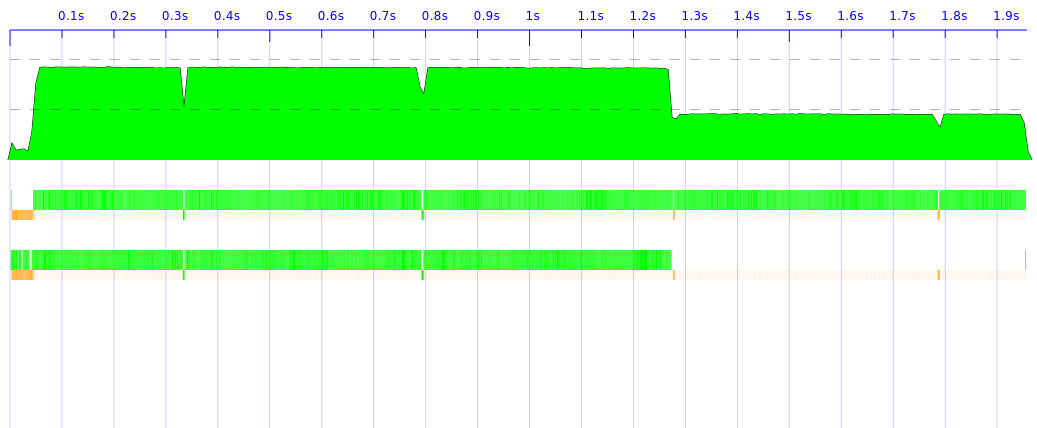
\includegraphics[scale=0.4]{sudoku2.png}
\end{center}
\caption{Sudoku2 ThreadScope profile}
\label{fig:sudoku2-threadscope}
\end{figure}

The ThreadScope profile is shown in \figref{sudoku2-threadscope};
this graph was generated by selecting ``export to PNG'' from
ThreadScope, so it includes the timeline graph only, and not the rest
of the ThreadScope GUI.  The $x$ axis of the graph is time, and there
are three horizontal bars showing how the program executed over time.
The topmost bar is known as the ``activity'' profile, and it shows how
many processors were executing Haskell code (as opposed to being idle
or garbage collecting) at a given point in time.  Then there is one
bar per processor, showing green when the processor is executing
Haskell code, and orange when it is garbage collecting.

As we can see from the graph, there is a period at the end of the run
where just one processor is executing, and the other one is idle
(except for participating in regular garbage collections, which is
necessary for GHC's parallel garbage collector).  This indicates that
our two parallel tasks are uneven: one takes much longer to execute
than the other, and so we are not making full use of our 2 processors,
which results in less than perfect speedup.

Why should the workloads be uneven?  After all, we divided the list in
two, and we know the sample input has an even number of problems.  The
reason for the unevenness is that each problem does not take the same
amount of time to solve, it all depends on the searching strategy used
by the Sudoku solver\footnote{in fact, we ordered the problems in the
  sample input so as to clearly demonstrate the problem.}.  This
illustrates an important distinction between two partitioning
strategies:

\begin{itemize}
\item \textbf{Static Partitioning}, which is the technique we used to
  partition the Sudoku problems here, consists of dividing the work
  according to some pre-defined policy (here, dividing the list
  equally in two).

\item \textbf{Dynamic Partitioning} instead tries to distribute the
  work more evenly, by dividing the work into smaller tasks and only
  assigning tasks to processors when they are idle.
\end{itemize}

The GHC runtime system supports automatic distribution of the parallel
tasks; all we have to do to achieve dynamic partitioning is divide the
problem into small enough tasks and the runtime will do the rest for
us.

The argument to @rpar@ is called a \emph{spark}.  The runtime collects
sparks in a pool and uses this as a source of work to do when there
are spare processors available, using a technique called \emph{work
  stealing} \cite{multicore-ghc-09}.  Sparks may be evaluated at some
point in the future, or they might not --- it all depends on whether
there is spare processor capacity available.  Sparks are very cheap to
create (@rpar@ essentially just adds a reference to the expression to
an array).

So, let's try using dynamic partitioning with the Sudoku problem.
First we define an abstraction that will let us apply a function to a
list in parallel, @parMap@:

\begin{numhaskell}
parMap :: (a -> b) -> [a] -> Eval [b]
parMap f [] = return []
parMap f (a:as) = do
   b <- rpar (f a)
   bs <- parMap f as
   return (b:bs)
\end{numhaskell}

\noindent This is rather like a monadic version of @map@, except that
we have used @rpar@ to lift the application of the function @f@ to the
element @a@ into the @Eval@ monad.  Hence, @parMap@ runs down the
whole list, eagerly creating sparks for the application of @f@ to each
element, and finally returns the new list.  When @parMap@ returns, it
will have created one spark for each element of the list.

We still need to evaluate the result list itself, and that is a
straightforward with @deep@:

\begin{haskell}
    evaluate $ deep $ runEval $ parMap solve grids
\end{haskell}

\noindent Running this new version\footnote{code sample @sudoku3.hs@}
yields more speedup:

{\small \begin{verbatim}
  Total time    3.55s  (  1.79s elapsed)
\end{verbatim}}

\noindent which we can calculate is equivalent to a speedup of
$3.06/1.79 = 1.7$, approaching the ideal speedup of 2.  Furthermore,
the GHC runtime system tells us how many sparks were created:

{\small \begin{verbatim}
  SPARKS: 1000 (1000 converted, 0 pruned)
\end{verbatim}}

\noindent we created exactly 1000 sparks, and they were all
\emph{converted} (that is, turned into real parallelism at runtime).
Sparks that are \emph{pruned} have been removed from the spark pool by
the runtime system, either because they were found to be already
evaluated, or because they were found to be not referenced by the rest
of the program, and so are deemed to be not useful.  We will discuss
the latter requirement in more detail in \secref{parlist}.

\begin{figure}
\begin{center}
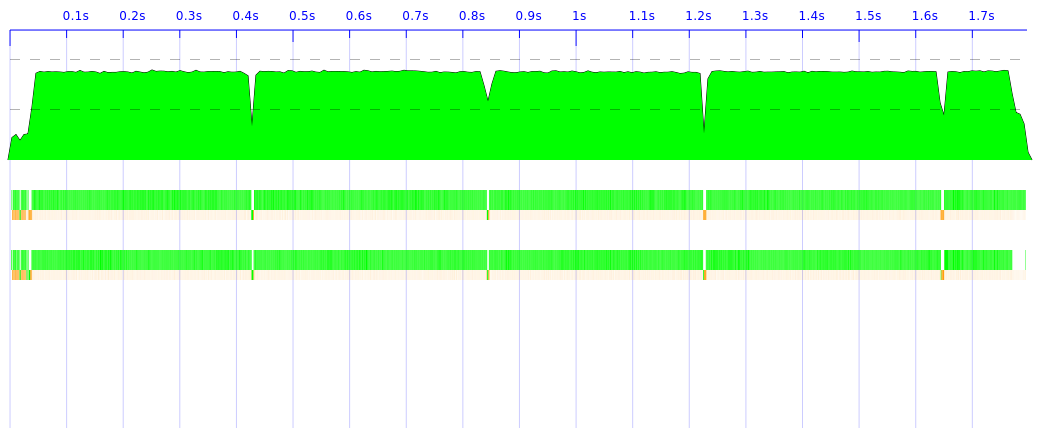
\includegraphics[scale=0.4]{sudoku3.png}
\end{center}
\caption{Sudoku3 ThreadScope profile}
\label{fig:sudoku3-threadscope}
\end{figure}

\begin{figure}
\begin{center}
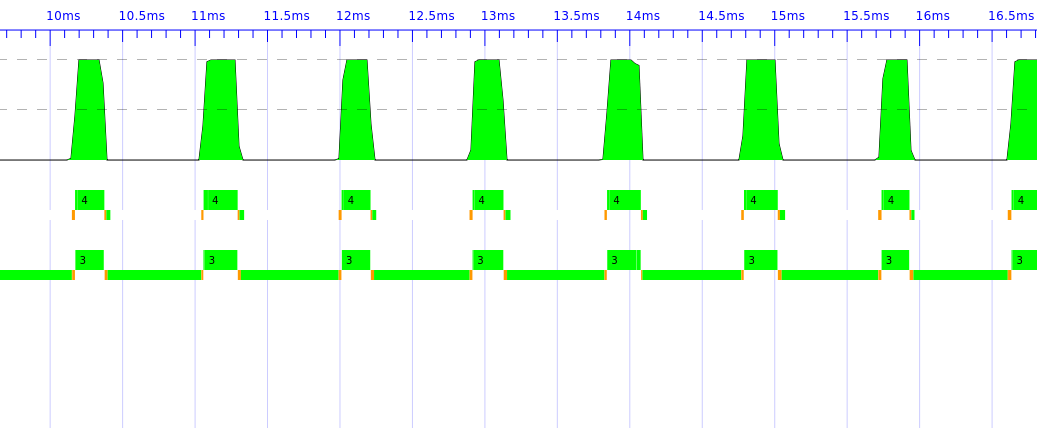
\includegraphics[scale=0.4]{sudoku3-zoom.png}
\end{center}
\caption{Sudoku3 (zoomed) ThreadScope profile}
\label{fig:sudoku3-zoom-threadscope}
\end{figure}

The threadscope profile looks much better
(\figref{sudoku3-threadscope}).  Furthermore, now that the runtime is
managing the work distribution for us, the program will automatically
scale to more processors.  On an 8 processor machine, for example:

{\small \begin{verbatim}
  Total time    4.46s  (  0.59s elapsed)
\end{verbatim}}

\noindent which equates to a speedup of 5.2 over the sequential
version.

If we look closely at the 2-processor profile there appears to be a
short section near the beginning where not much work is happening.  In
fact, zooming in on this section in ThreadScope
(\figref{sudoku3-zoom-threadscope}) reveals that both processors
are working, but most of the activity is garbage collection, and only
one processor is performing most of the garbage collection work.  In
fact, what we are seeing here is the program reading the input file
(lazilly) and dividing it into lines, driven by the demand of @parMap@
which traverses the whole list of lines.

Since reading the file and dividing it into lines is a sequential
activity anyway, we could force it to happen all at once before we
start the main computation, by adding

\begin{haskell}
    evaluate (length grids)
\end{haskell}

\noindent (see code sample @sudoku4.hs@).  This makes no difference to
the overall runtime, but it divides the execution into sequential and
parallel parts, as we can see in ThreadScope
(\figref{sudoku4-threadscope}).

\begin{figure}
\begin{center}
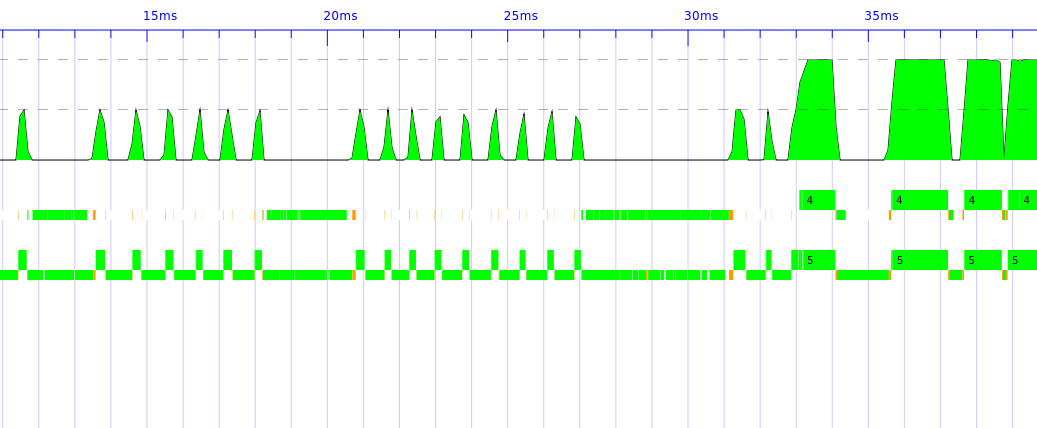
\includegraphics[scale=0.4]{sudoku4.png}
\end{center}
\caption{Sudoku4 ThreadScope profile}
\label{fig:sudoku4-threadscope}
\end{figure}

Now, we can read off the portion of the runtime that is sequential:
33ms.  When we have a sequential portion of our program, this affects
the maximum parallel speedup that is achievable, which we can
calculate using Amdahl's law.  Amdahl's law gives the maximum
achievable speedup as the ratio

\[
  \frac{1}{(1 - P) + \frac{P}{N}}
\]

\noindent where $P$ is the portion of the runtime that can be
parallelised, and $N$ is the number of processors available.  In our
case, $P$ is $(3.06-0.033)/3.06 = 0.9892$, and the maximum speedup is
hence 1.98.  The sequential fraction here is too small to make a
significant impact on the theoretical maximum speedup with 2
processors, but when we have more processors, say 64, it becomes much
more important: $1 / ((1-0.989) + 0.989/64) = 38.1$.  So no matter
what we do, this tiny sequential part of our program will limit the
maximum speedup we can obtain with 64 processors to 38.1.  In fact,
even with 1024 cores we could only achieve around 84 speedup, and it
is impossible to achieve a speedup of 91 no matter how many cores we
have.  Amdahl's law tells us that not only does parallel speedup
become harder to achieve the more processors we add, in practice most
programs have a theoretical maximum amount of parallelism.

\Subsection{strategies}{Evaluation Strategies}

Evaluation Strategies \cite{trinder:strategies,seq-no-more} is an abstraction
layer built on top of the @Eval@ monad that allows larger parallel
specifications to be built in a compositional way.  Furthermore
Strategies allow parallel coordination to be described in a modular
way, separating parallelism from the algorithm to be parallelised.

A Strategy is merely a function in the @Eval@ monad that takes a value
of type @a@ and returns the same value:

\begin{haskell}
type Strategy a = a -> Eval a
\end{haskell}

\noindent Strategies are identity functions; that is, the value
returned by a @Strategy@ is observably equivalent to the value it was
passed.  Unfortunately the library cannot statically guarantee this
property for user-defined @Strategy@ functions, but it holds for the
@Strategy@ funcitons and combinators provided by the
@Control.Parallel.Strategies@ module.

We have already seen some simple Strategies, @rpar@ and @rseq@,
although we can now give their types in terms of @Strategy@:

\begin{haskell}
rseq :: Strategy a
rpar :: Strategy a
\end{haskell}

\noindent There are two further members of this family:

\begin{haskell}
r0 :: Strategy a
r0 x = return x

rdeepseq :: NFData a => Strategy a
rdeepseq x = rseq (deep x)
\end{haskell}

\noindent @r0@ is the @Strategy@ that evaluates nothing, and
@rdeepseq@ is the @Strategy@ that evaluates the entire structure of
its argument (it can be defined in terms of @deep@ that we saw
eariler).

We have some simple ways to build Strategies, but how is a Strategy
actually \emph{used}?  A @Strategy@ is just a function yielding a
computation in the @Eval@ monad, so we could use @runEval@.  For
example, applying the strategy @s@ to a value @x@ would be simply
@runEval (s x)@.  This is such a common pattern that the
Strategies library gives it a name, @using@:

\begin{haskell}
using :: a -> Strategy a -> a
x `using` s = runEval (s x)
\end{haskell}

\noindent @using@ takes a value of type @a@, a Strategy for @a@, and
applies the Strategy to the value.  The identity property for
@Strategy@ gives us that

{\small \begin{verbatim}
  x `using` s == x
\end{verbatim}}

\noindent which is a significant benefit of Strategies: every
occurrence of @`using` s@ can be deleted without affecting the
semantics.  Strictly speaking there are two caveats to this property.
Firstly, as mentioned earlier, user-defined @Strategy@ functions migh0t
not satisfy the identity property.  Secondly, @x `using` s@ might be
less defined than @x@, because it evaluates more structure of @x@ than
the context does.  So deleting @`using` s@ might have the effect of
making the program terminate with a result when it would previously
throw an exception or fail to terminate.  Making programs more defined
is generally considered to be a somewhat benign change in semantics
(indeed, GHC's optimiser can also make programs more defined under
certain conditions), but nevertheless it is a change in semantics.

\Subsubsection{parlist}{A Strategy for evaluating a list in parallel}

In \secref{par-eval} we defined a function @parMap@ that would map a
function over a list in parallel.  We can think of @parMap@ as a
composition of two parts:

\begin{itemize}
\item The algorithm: @map@
\item The parallelism: evaluating the elements of a list in parallel
\end{itemize}

\noindent and indeed with Strategies we can express it exactly this
way:

\begin{haskell}
parMap f xs = map f xs `using` parList rseq
\end{haskell}

\noindent The benefits of this approach are two-fold: not only does it
separate the algorithm from the parallelism, but it also \emph{reuses}
@map@, rather than re-implementing a parallel version.

The @parList@ function is a Strategy on lists, defined as follows:

\begin{haskell}
parList :: Strategy a -> Strategy [a]
parList strat []     = return []
parList strat (x:xs) = do
  x'  <- rpar (x `using` strat)
  xs' <- parList strat xs
  return (x':xs')
\end{haskell}

\noindent (in fact, @parList@ is already provided by
@Control.Parallel.Strategies@ so you don't have to define it yourself,
but we are using its implementation here as an illustration).

The @parList@ function is a \emph{paramterised} Strategy, that is, it
takes as an argument a Strategy on values of type @a@, and returns a
Strategy for lists of @a@.  This illustrates another important aspect
of Strategies: they are compositional, in the sense that we can build
larger strategies by composing smaller reusable components.  Here,
@parList@ describes a family of Strategies on lists that evaluate the
list elements in parallel.

On line 4, @parList@ calls @rpar@ to create a spark to evaluate the
current element of the list.  Note that the spark evaluates
@(x `using` strat)@: that is, it applies the argument Strategy @strat@ to
the list element @x@.

As @parList@ traverses the list sparking list elements, it remembers
each value returned by @rpar@ (bound to @x'@), and constructs a new
list from these values.  Why?  After all, this seems to be a lot of
trouble to go to, because it means that @parList@ is no longer
\emph{tail-recursive} --- the recursive call to @parList@ is not the
last operation in the @do@ on its right-hand side, and so @parList@
will require stack space linear in the length of the input list.

Couldn't we write a tail-recursive version instead?  For example:

\begin{haskell}
parList :: Strategy a -> Strategy [a]
parList strat xs = do go xs; return xs
  where go [] = return ()
        go (x:xs) = do
           rpar (x `using` strat)
           go xs
\end{haskell}

\noindent This typechecks, after all, and seems to call @rpar@ on each
list element as required.

\begin{figure}
\begin{center}
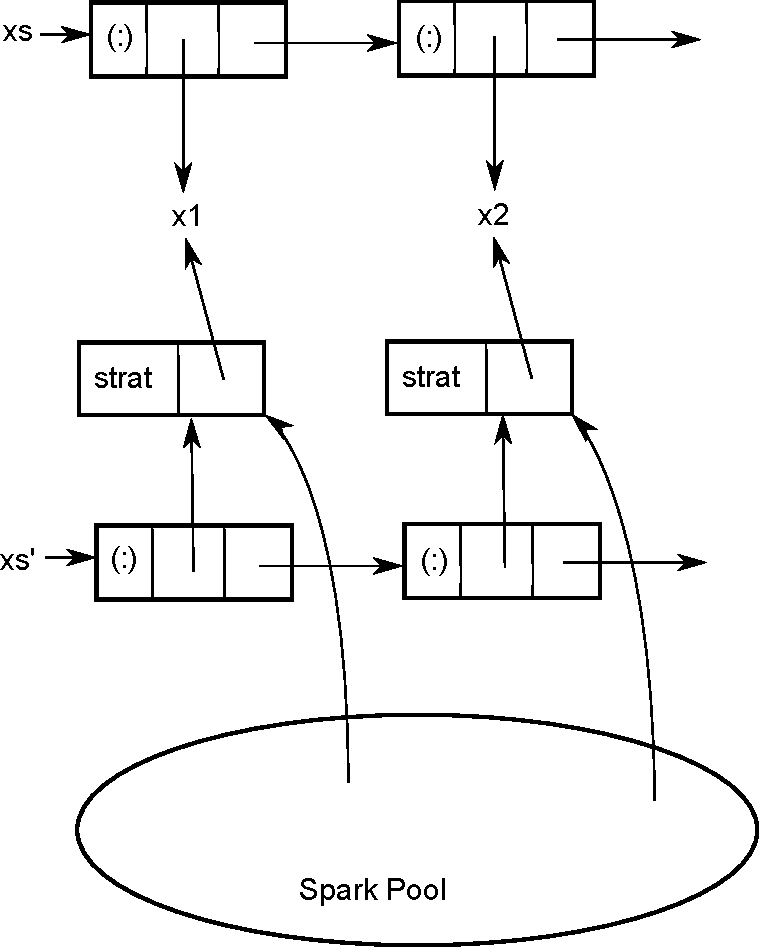
\includegraphics[scale=0.6]{parlist1.pdf}
\end{center}
\caption{\texttt{parList} heap structures}
\label{fig:parlist-heap}
\end{figure}

The difference is subtle but important, and is best understood via a
diagram (\figref{parlist-heap}).  At the top of the diagram we have
the input list @xs@: a linked list of cells, each of which points to a
list element (@x1@, @x2@, and so forth).  At the bottom of the diagram
is the \emph{spark pool}, the runtime system data structure that
stores references to sparks in the heap.  The other structures in the
diagram are built by @parList@ (the first version).  Each @strat@ box
represents @(x `using` strat)@ for an element of the original list
@x@, and @xs'@ is the linked list of cells in the output list.  The
spark pool contains pointers to each of the @strat@ boxes; these are
the pointers created by the @rpar@ calls.

Now, the spark pool only retains references to objects that are
required by the program.  If the runtime finds that the spark pool
contains a reference to an object that the program will never use,
then the reference is dropped, and any potential parallelism it
represented is lost.  This behaviour is a deliberate policy; if it
weren't this way, then the spark pool could retain data indefintely,
causing a space leak (details can be found in \citet{seq-no-more}).

This is the reason for the list @xs'@.  Suppose we did not build the
new list @xs'@, as in the tail-recursive version of @parList@ above.
Then, the only reference to each @strat@ box in the heap would be from the
spark pool, and hence the runtime would automatically sweep all those
references from the spark pool, discarding the parallelism.  Hence we
build a new list @xs'@, so that the program can retain references to
the sparks for as long as it needs to.

This behaviour has another benefit: suppose that under some
circumstances the program does not need the entire list.  If the
program simply forgets the unused remainder of the list, the runtime
system will clean up the unreferenced sparks from the spark pool, and
will not waste any further parallel processing resources on evaluating
those sparks.  The extra parallelism in this case is termed
\emph{speculative}, because it is not necessarily required, and the
runtime will automatically discard speculative tasks that it can prove
will never be required - a useful property!

While the runtime system's discarding of unreferenced sparks is
certainly useful in some cases, it can be tricky to work with, because
there is no language-level support for catching mistakes.  Fortunately
the runtime system will tell us if it garbage collects unreferenced
sparks; for example:

{\small \begin{verbatim}
  SPARKS: 144 (0 converted, 144 pruned)
\end{verbatim}}

\noindent A large number of sparks being ``pruned'' is a good
indication that sparks are being removed from the spark pool before
they can be used for parallelism.  Sparks can be pruned for several
reasons:

\begin{itemize}
\item The spark was a \emph{dud}: it was already evaluated at the
  point it was sparked.
\item The spark \emph{fizzled}: it was evaluated by some other thread
  before it could be evaluated in parallel.
\item The spark was garbage collected, as described above.
\end{itemize}

In fact, GHC from version 7.2.1 onwards separates these different
classifications in its output from @+RTS -s@:

{\small \begin{verbatim}
  SPARKS: 144 (0 converted, 0 dud, 144 GC'd, 0 fizzled)
\end{verbatim}}

\noindent Unless you are using speculation, then a non-zero figure for
GC'd sparks is probably a bad sign.

All of the combinators in the library @Control.Parallel.Strategies@
behave correctly with respect to retaining references to sparks when
necessary.  So the rules of thumb for not tripping up here are:

\begin{itemize}
\item Use @using@ to apply strategies: it encourages the right
  pattern, in which the program uses the results of applying the
  Strategy.
\item When writing your own @Eval@-monad code, remember to bind the
  result of @rpar@, and use its result.
\end{itemize}

\Subsubsection{using-parlist}{Using \texttt{parList}: the K-Means problem}

The @parList@ Strategy covers a wide range of uses for parallelism in
typical Haskell programs; in many cases, a single @parList@ is all
that is needed to expose sufficient parallelism.

Returning to our Sudoku solver from \secref{par-eval} for a moment,
instead of our own hand-written @parMap@, we could have used
@parList@:

\begin{haskell}
    evaluate $ deep $ map solve grids `using` parList rseq
\end{haskell}

\begin{figure}
\begin{center}
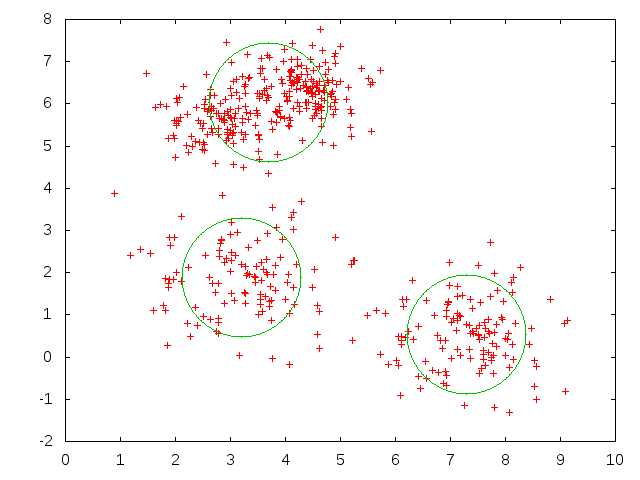
\includegraphics[scale=0.6]{kmeans-example.png}
\end{center}
\caption{The K-Means problem}
\label{fig:kmeans-example}
\end{figure}

Let's look at a slightly more involved example.  In the K-Means
problem, the goal is to partition a set of data points into clusters.
Finding an optimal solution to the problem is NP-hard, but there exist
several heuristic techniques that do not guarantee to find an optimal
solution, but work well in practice.  For example, given the data
points shown in \figref{kmeans-example}, the algorithm should discover
the clusters indicated by the circles.  Here we have only shown the
locations of the clusters, partitioning the points is achieved by
simply finding the closest cluster to each point.

The most well-known heuristic technique is Lloyd's algorithm, which
finds a solution by iteratively improving an initial guess, as
follows:

\begin{enumerate}
\item Pick an initial set of clusters by randomly assigning each point
  in the data set to a cluster.
\item Find the centroid of each cluster (the average of all the points
  in the cluster).
\item Assign each point to the cluster to which it is closest, this
  gives a new set of clusters.
\item Repeat steps 2--3 until the set of clusters stabilises.
\end{enumerate}

Of course the algorithm works in any number of dimensions, but we will
use 2 for ease of visualisation.

A complete Haskell implementation can be found in the directory
@kmeans@ in the sample code; \figref{kmeans-code} shows the core of
the algorithm.

\begin{figure}
\begin{numhaskell}
data Vector = Vector Double Double

addVector :: Vector -> Vector -> Vector
addVector (Vector a b) (Vector c d) = Vector (a+c) (b+d)

data Cluster = Cluster
               {
                  clId    :: !Int,
                  clCount :: !Int,
                  clSum   :: !Vector,
                  clCent  :: !Vector
               }

sqDistance :: Vector -> Vector -> Double
sqDistance (Vector x1 y1) (Vector x2 y2)
  = ((x1-x2)^2) + ((y1-y2)^2)

makeCluster :: Int -> [Vector] -> Cluster
makeCluster clid vecs
  = Cluster { clId = clid,
              clCount = count,
              clSum = vecsum,
              clCent = centre }
  where
   vecsum@(Vector a b)  = foldl' addVector (Vector 0 0) vecs
   centre = Vector (a / fromIntegral count)
                   (b / fromIntegral count)
   count = fromIntegral (length vecs)

-- assign each vector to the nearest cluster centre
assign :: Int -> [Cluster] -> [Vector] -> Array Int [Vector]
assign nclusters clusters points =
  accumArray (flip (:)) [] (0, nclusters-1)
     [ (clId (nearest p), p) | p <- points ]
  where
    nearest p = fst $ minimumBy (compare `on` snd)
                        [ (c, sqDistance (clCent c) p)
                        | c <- clusters ]

-- compute clusters from the assignment
makeNewClusters :: Array Int [Vector] -> [Cluster]
makeNewClusters arr =
  filter ((>0) . clCount) $
     [ makeCluster i ps | (i,ps) <- assocs arr ]

step :: Int -> [Cluster] -> [Vector] -> [Cluster]
step nclusters clusters points =
   makeNewClusters (assign nclusters clusters points)
\end{numhaskell}

\caption{Haskell code for K-Means}
\label{fig:kmeans-code}
\end{figure}

A data point is represented by the type @Vector@, which is just a pair
of @Double@s.  Clusters are represented by the type @Cluster@, which
contains its number, the count of points assigned to this cluster, the
sum of the @Vector@s in the cluster, and its centre.  Everything about
the cluster except its number is derivable from the set of points in
the cluster; this is expressed by the function @makeCluster@.
Essentially @Cluster@ caches various information about a cluster, and
the reason we need to cache these specific items will become clear
shortly.

The function @assign@ implements step 2 of the algorithm, assigning
points to clusters.  The @accumArray@ function is particularly useful
for this kind of bucket-sorting task.  The function @makeNewClusters@
implements step 3 of the algorithm, and finally @step@ combines
@assign@ and @makeNewClusters@ to implement one complete iteration.

To complete the algorithm we need a driver to repeatedly apply the
@step@ function until convergence.  The function @kmeans_seq@, below,
implements this:

\begin{haskell}
kmeans_seq :: Int -> [Vector] -> [Cluster] -> IO [Cluster]
kmeans_seq nclusters points clusters = do
  let
      loop :: Int -> [Cluster] -> IO [Cluster]
      loop n clusters | n > tooMany = return clusters
      loop n clusters = do
        hPrintf stderr "iteration %d\n" n
        hPutStr stderr (unlines (map show clusters))
        let clusters' = step nclusters clusters points
        if clusters' == clusters
           then return clusters
           else loop (n+1) clusters'
  --
  loop 0 clusters
\end{haskell}

How can this algorithm be parallelised?  One place that looks
straightforward to parallelise is the @assign@ function, since it is
essentially just a @map@ over the points.  However, that doesn't get
us very far: we cannot parallelise @accumArray@ directly, so we would
have to do multiple @accumArray@s and combine the results, and
combining elements would mean an extra list append.  The
@makeNewClusters@ operation parallelises easily, but only in so far as
each @makeCluster@ is independent of the others; typically the number
of clusters is much smaller than the number of points (e.g. a few
clusters to a few hundred thousand points), so we don't gain much
scalability by parallelising @makeNewClusters@.

We would like a way to parallelise the problem at a higher level.
That is, we would like to divide the set of points into chunks, and
process each chunk in parallel, somehow combining the results.  In
order to do this, we need a @combine@ function, such that

{\small \begin{verbatim}
 points == as ++ bs
   ==>
 step n cs points == step n cs as `combine` step n cs bs
\end{verbatim}}

Fortunately defining @combine@ is not difficult.  A cluster is a set
of points, from which we can compute a centroid.  The intermediate
values in this calcuation are the sum and the count of the data
points.  So a combined cluster can be computed from two independent
sub-clusters by taking the sum of these two intermediate values, and
re-computing the centroid from them.  Since addition is associative
and commutative, we can compute sub-clusters in any way we wish and
then combine them in this way.

Our Haskell code for combining two clusters is as follows:

\begin{haskell}
combineClusters c1 c2 =
  Cluster {clId = clId c1,
           clCount = count,
           clSum = vecsum,
           clCent = Vector (a / fromIntegral count)
                           (b / fromIntegral count)}
  where count = clCount c1 + clCount c2
        vecsum@(Vector a b)  = addVector (clSum c1) (clSum c2)
\end{haskell}

\noindent In general, however, we will be processing $N$ chunks of the
data space independently, each of which returns a set of clusters.  So
we need to reduce the $N$ sets of sets of clusters to a single set.
This is done with another @accumArray@:

\begin{haskell}
reduce :: Int -> [[Cluster]] -> [Cluster]
reduce nclusters css =
  concatMap combine $ elems $
    accumArray (flip (:)) [] (0,nclusters)
       [ (clId c, c) | c <- concat css]
 where
  combine [] = []
  combine (c:cs) = [foldr combineClusters c cs]
\end{haskell}

Now, the parallel K-Means implementation can be expressed as an
application of @parList@ to invoke @step@ on each chunk, followed by a
call to @reduce@ to combine the results from the chunks:

\begin{numhaskell}
kmeans_par :: Int -> Int -> [Vector] -> [Cluster]
           -> IO [Cluster]
kmeans_par chunks nclusters points clusters = do
  let chunks = split chunks points
  let
      loop :: Int -> [Cluster] -> IO [Cluster]
      loop n clusters | n > tooMany = return clusters
      loop n clusters = do
        hPrintf stderr "iteration %d\n" n
        hPutStr stderr (unlines (map show clusters))
        let
             new_clusterss =
                map (step nclusters clusters) chunks
                   `using` parList rdeepseq

             clusters' = reduce nclusters new_clusterss

        if clusters' == clusters
           then return clusters
           else loop (n+1) clusters'
  --
  loop 0 clusters
\end{numhaskell}

\noindent the only difference from the sequential implementation is at
lines 11--14, where we map @step@ over the chunks applying the
@parList@ strategy, and then call @reduce@.

Note that there's no reason the number of chunks has to be related to
the number of processors; as we saw earlier, it is better to produce
plenty of sparks and let the runtime schedule them automatically,
since this should enable the program to scale over a wide range of
processors.

\figref{kmeans-results} shows the speedups obtained by this
implementation for a randomly-generated data set consisting of 4
clusters with a total of approximately 170000 points in 2-D space.
The data was generated using the Haskell @normaldistribution@ package
in order to generate realistically clustered points\footnote{The
  program used to generate the data is provided as
  @kmeans/GenSamples.hs@ in the sample code distribution, and the
  sample data we used for this benchmark is provided in the files
  @kmeans/points.bin@ and @kmeans/clusters@ (the @GenSamples@ program
  will overwrite these files, so be careful if you run it!)}.  For this
benchmark we used 1000 for the @chunk@ parameter to @kmeans_par@.

The results show the algorithm scaling reasonably well up to 6 cores,
with a drop in performance at 8 cores.  We leave it as an exercise for
the reader to analyse the performance and improve it further!

\begin{figure}
\begin{center}
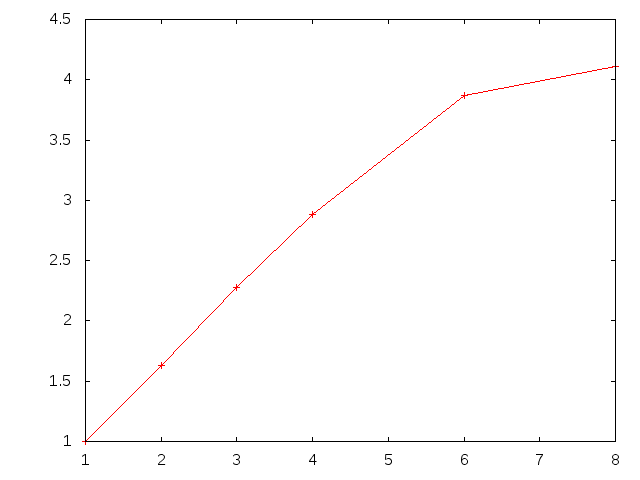
\includegraphics[scale=0.4]{kmeans-results.png}
\end{center}
\caption{Scaling of parallel K-Means}
\label{fig:kmeans-results}
\end{figure}

\Subsubsection{strat-further}{Further Reading}

We have barely scratched the surface of the possibilities with the
@Eval@ monad and Strategies here.  Topics that we have not covered
include:

\begin{itemize}
\item Sequential strategies, which allow greater control over the
  specification of \emph{evaluation degree} than is provided by @rseq@
  and @rdeepseq@.  See the documentation for the @Control.Seq@ module\footnote{\url{http://hackage.haskell.org/packages/archive/parallel/3.1.0.1/doc/html/Control-Seq.html}}.
\item Clustering, which allows greater control over granularity.
\item @parBuffer@: a combinator for parallelising lazy streams.
\end{itemize}

To learn more, we recommend the following resources:

\begin{itemize}
\item The documentation for the @Control.Parallel.Strategies@ module\footnote{\url{http://hackage.haskell.org/packages/archive/parallel/3.1.0.1/doc/html/Control-Parallel-Strategies.html}}.
\item \citet{seq-no-more}, which explains the motivation behind the
  design and implementation of @Eval@ and Strategies.
\item \citet{pjsingh-tutorial}, an earlier tutorial covering
  basic parallelism in Haskell (beware: this dates from before the
  introduction of the @Eval@ monad).
\item \citet{trinder:strategies}, which has a wide range of examples.
  However beware: this paper is based on the earlier version of
  Strategies, and some of the examples may no longer work due to the
  new GC behaviour on sparks; also some the names of functions and
  types in the library have since changed.
\end{itemize}

\Subsection{monad-par}{Dataflow parallelism: the \texttt{Par} monad}

Sometimes there is a need to be \emph{more explicit} about
dependencies and task boundaries than it is possible to be with @Eval@
and Strategies.  In these cases the usual recourse is to Concurrent
Haskell, where we can fork threads and be explicit about which thread
does the work.  However, that approach throws out the baby with the
bathwater: determinism is lost.  The programming model we introduce in
this section fills the gap between Strategies and Concurrent Haskell:
it is explicit about dependencies and task boundaries, but without
sacrificing determinism.  Furthermore the programming model has some
other interesting benefits: for example, it is implemented entirely as
a Haskell library and the implementation is readily modified to
accommodate alternative scheduling strategies.

As usual, the interface is based around a monad, this time called @Par@:

\begin{haskell}
  newtype Par a
  instance Functor Par
  instance Applicative Par
  instance Monad Par

  runPar :: Par a -> a
\end{haskell}

\noindent As with the @Eval@ monad, the @Par@ monad returns a pure
result.  However, use @runPar@ with care: internally it is much more
expensive than @runEval@, because (at least in the current
implementation) it will fire up a new scheduler instance consisting of
one worker thread per processor.  Generally speaking the program
should be using @runPar@ to schedule large-sale parallel tasks.

The purpose of @Par@ is to introduce parallelism, so we need a way to
create parallel tasks:

\begin{haskell}
  fork :: Par () -> Par ()
\end{haskell}

\noindent @fork@ does exactly what you would expect: the computation
passed as the argument to @fork@ (the ``child'') is executed
concurrently with the current computation (the ``parent'').

Of course, @fork@ on its own isn't very useful; we need a way to
communicate results from the child of @fork@ to the parent, or in
general between two parallel @Par@ computations.  Communication is
provided by the @IVar@ type\footnote{@IVar@ is so-called because it is an implementation of
I-Structures, a concept from the Parallel Haskell variant pH} and its operations:

\begin{haskell}
  data IVar a  -- instance Eq

  new :: Par (IVar a)
  put :: NFData a => IVar a -> a -> Par ()
  get :: IVar a -> Par a
\end{haskell}

\noindent @new@ creates a new @IVar@, which is initially empty; @put@
fills an @IVar@ with a value, and @get@ retrieves the value of an
@IVar@ (waiting until a value has been @put@ if necessary).  Multiple
@put@s to the same @IVar@ result in an error.

The @IVar@ type is a relative of the @MVar@ type that we shall see
later in the context of Concurrent Haskell (\secref{mvars}), the main
difference being that an @IVar@ can only be written once.  An @IVar@
is also like a \emph{future} or \emph{promise}, concepts that may be
familiar from other parallel or concurrent languages.

Together, @fork@ and @IVar@s together allow the construction of
\emph{dataflow} networks.  The nodes of the network are created by
@fork@, and edges connect a @put@ with each @get@ on that @IVar@.  For
example, suppose we have the following four functions:

\begin{haskell}
f :: In -> A
g :: A -> B
h :: A -> C
j :: (B,C) -> Out
\end{haskell}

\noindent Composing these functions forms the following dataflow graph:

\begin{center}
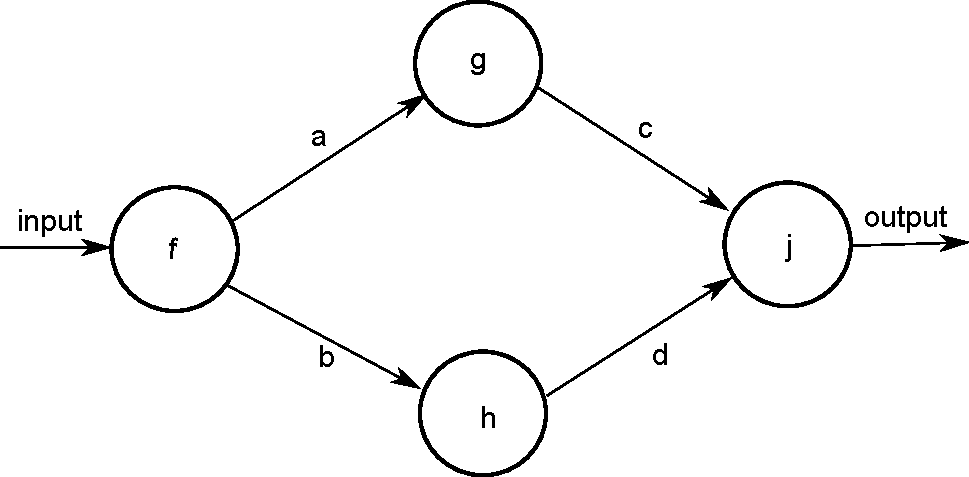
\includegraphics[scale=0.6]{dataflow.pdf}
\end{center}

There are no sequential dependencies between @f@ and @g@, so they
could run in parallel.  In order to take advantage of the parallelism
here, all we need to do is express the graph in the @Par@ monad:

\begin{haskell}
do
   [ia,ib,ic] <- replicateM 4 new

   fork $ do x <- get in
             put ia (f x)

   fork $ do a <- get ia
             put ib (g a)

   fork $ do a <- get ia
             put ic (h a)

   fork $ do b <- get ib
             c <- get ic
             put out (j b c)
\end{haskell}

\noindent For each edge in the graph we make an @IVar@ (here @ia@,
@ib@ and so on).  For each node in the graph we call @fork@, and the
code for each node calls @get@ on each input, and @put@ on each output
of the node.  The order of the @fork@ calls is irrelevant --- the
@Par@ monad will execute the graph, resolving the dependencies at
runtime.

While the @Par@ monad is particularly suited to expressing dataflow
networks, it can also express other common patterns too.  For example,
we can build an equivalent of the @parMap@ combinator that we saw
earlier in \secref{par-eval}.  First, we build a simple abstraction
for a parallel computation that returns a result:

\begin{haskell}
spawn :: NFData a => Par a -> Par (IVar a)
spawn p = do
  i <- new
  fork (do x <- p; put i x)
  return i
\end{haskell}

\noindent The @spawn@ function forks a computation in parallel, and
returns an @IVar@ that can be used to wait for the result.

Now, parallel map consists of calling @spawn@ to apply the function to
each element of the list, and then waiting for all the results:

\begin{haskell}
parMapM :: NFData b => (a -> Par b) -> [a] -> Par [b]
parMapM f as = do
  ibs <- mapM (spawn . f) as
  mapM get ibs
\end{haskell}

\noindent Note that there are a couple of differences between this and
the @Eval@ monad @parMap@.  First, the function argument returns its
result in the @Par@ monad; of course it is easy to lift an arbitrary
pure function to this type, but the monadic version allows the
computation on each element to produce more parallel tasks, or augment
the dataflow graph in other ways.  Second, @parMapM@ waits for all the
results.  Depending on the context, this may or may not be the most
useful behaviour, but of course it is easy to define the other version
if necessary.

\Subsubsection{monad-par-infer}{A parallel type inferencer}

In this section we will parallelise a type inference engine using the
@Par@ monad.  Type inference is a natural fit for the dataflow model,
because we can consider each binding to be a node in the graph, and
the edges of the graph carry inferred types from bindings to usage
sites in the program.

For example, consider the following program set of bindings that we
want to infer types for:

{\small \begin{verbatim}
  f = ...
  g = ... f ...
  h = ... f ...
  j = ... g ... h ...
\end{verbatim}}

This pattern gives rise to a dataflow graph with exactly the shape of
the example 4-node graph in the previous section: after we have
inferred a type for @f@, we can use that type to infer types for @g@
and @h@ (in parallel), and once we have the types for @g@ and @h@ we
can infer a type for @j@.

Building a dataflow graph for the type inference problem allows the
maximum amount of parallelism to be extracted from the type inference
process.  The actual amount of parallelism present depends on the
structure of the input program, however.

The parallel type inferencer can be found in the directory @parinfer@
of the code samples, and is derived from a (rather ancient) type
inference engine written by Phil Wadler.  The types from the inference
engine that we will need to work with are as follows:

\begin{numhaskell}
type VarId = String -- variables

data Env -- environment for the type inferencer

-- build environments
makeEnv :: [(VarId,Type)] -> Env

data MonoType -- monomorphic types
data PolyType -- polymorphic types

-- Terms in the input program
data Term = Let VarId Term Term | ...
\end{numhaskell}

The input to this type inferencer is a single @Term@ which may contain
@let@ bindings, and so to parallelise it we will strip off the outer
@let@ bindings and typecheck them in parallel.  The inner term will be
typechecked using the ordinary sequential inference engine.  We could
have a more general parallel type inference algorithm by always
typechecking a @let@ binding in parallel with the body, rather than
just for the outer @let@s, but that would require threading the @Par@
monad through the type inference engine, so for this simple example we
are only parallelising inference for the outer bindings.

We need two functions from the inference engine.  First, a way to
infer a polymorphic type for the right-hand side of a binding:

\begin{haskell}
inferTopRhs :: Env -> Term -> PolyType
\end{haskell}

\noindent and secondly, a way to run the inference engine on an
arbitrary term:

\begin{haskell}
inferTopTerm :: Env -> Term -> MonoType
\end{haskell}

The basic idea is that while the sequential inference engine uses an
@Env@ that maps @VarId@s to @PolyType@s, the parallel part of the
inference engine will use an environment that maps @VarId@s to
@IVar PolyType@, so that we can @fork@ the inference engine for a
given binding, and then wait for its result later\footnote{We are
  ignoring the possibility of type errors here; in a real
  implementation the @IVar@ would probably contain an @Either@ type
  representing either the inferred type or an error,}.  The environment
for the parallel type inferencer is called @TopEnv@:

\begin{haskell}
type TopEnv = Map VarId (IVar PolyType)
\end{haskell}

All that remains is to write the top-level loop.  We will write a
function @inferTop@ with the following type:

\begin{haskell}
inferTop :: TopEnv -> Term -> Par MonoType
\end{haskell}

\noindent There are two cases to consider.  First, when we are looking at a
@let@ binding:

\begin{numhaskell}
inferTop topenv (Let x u v) = do
    vu <- new

    fork $ do
      let fu = Set.toList (freeVars u)
      tfu <- mapM (get . fromJust . flip Map.lookup topenv) fu
      let aa = makeEnv (zip fu tfu)
      put vu (inferTopRhs aa u)

    inferTop (Map.insert x vu topenv) v
\end{numhaskell}

\noindent On line 2 we create the @IVar@ to hold the result, @vu@.  Lines
4--8 implement the typechecking for the binding:

\begin{itemize}
\item [4] We @fork@ here, so that the binding is typechecked in
  parallel,
\item [5] Find the @IVar@s corresponding to the free variables of the right-hand side
\item [6] Call @get@ for each of these, thus waiting for the
  typechecking of the binding corresponding to each free variable
\item [7] Make a new @Env@ with the types we obtained on line 6
\item [8] Call the type inferencer for the right-hand side, put the
  result in the @IVar@ @vu@.
\end{itemize}

The main computation continues (line 10) by typechecking the body of
the @let@ in an environment in which the bound variable @x@ is mapped
to the @IVar@ @vu@.

The other case of @inferTop@ handles all other expression constructs:

\begin{numhaskell}
inferTop topenv t = do
    let (vs,ivs) = unzip (Map.toList topenv)
    tvs <- mapM get ivs
    let aa = makeEnv (zip vs tvs)
    return (inferTopTerm aa t)
\end{numhaskell}

\noindent This case is straightforward: just call @get@ to obtain the
inferred type for for each binding in the @TopEnv@, construct an
@Env@, and call the sequential inferencer on the term @t@.

This parallel implementation works quite nicely.  For example, the
input file below (with some duplicate bindings elided, the full
version is in the file @parinfer/example/in@) defines an expression in
which there are two parallel branches to infer, one represented by
the sequence of @let@ bindings for @x@ (each successive binding for
@x@ shadows the previous), and the other branch represented by the
sequence of @let@ bindings for @y@:

{\small \begin{verbatim}
let id = \x.x in
    let x = \f.f id id in
    let x = \f . f x x in
    let x = \f . f x x in
    let x = \f . f x x in
    ...
    let x = let f = x in \z . z in
    let y = \f.f id id in
    let y = \f . f y y in
    let y = \f . f y y in
    let y = \f . f y y in
    ...
    let x = let f = y in \z . z in
    \f. let g = \a. a x y in f
\end{verbatim}}

\noindent With one processor:

{\small \begin{verbatim}
$ ./infer <./example.in +RTS -s
  ...
  Total time    1.13s  (  1.12s elapsed)
\end{verbatim}}

\noindent and with two processors:

{\small \begin{verbatim}
$ ./infer <./example.in +RTS -s -N2
  ,..
  Total time    1.19s  (  0.60s elapsed)
\end{verbatim}}

\noindent representing a speedup of 1.87.

\Subsubsection{monad-par-reflections}{The \texttt{Par} monad compared
  to Strategies}

We have presented two different parallel programming models, each with
advantages and disadvantages.  Below we summarise the trade-offs so
that you can make an informed decision for a given task as to which is
likely to be the best choice:

\begin{itemize}
\item Using Strategies and the @Eval@ monad requires some
  understanding of the workings of lazy evaluation.  Newcomers often
  find this hard, and diagnosing problems can be difficult.  This is
  part of the motivation for the @Par@ monad: it makes all
  dependencies explicit, effectively replacing lazy evaluation with
  explicit @put@/@get@ on @IVar@s.  While this is certainly more
  verbose, it is less fragile and easier to work with.

  Programming with @rpar@ requires being careful about retaining
  references to sparks to avoid them being garbage collected; this can
  be subtle and hard to get right in some cases.  The @Par@ monad has
  no such requirements, although it does not support speculative
  parallelism in the sense that @rpar@ does: speculative paralelism
  in the @Par@ monad is always executed.

\item Strategies allow a separation between algorithm and parallelism,
  which allows more reuse in some cases.

\item The @Par@ monad requires threading the monad throughout a
  computation which is to be parallelised.  For example, to
  parallelise the type inference of all @let@ bindings in the example
  above would have required threading the @Par@ monad through the
  inference engine (or adding @Par@ to the existing monad stack),
  which might be impractical.  @Par@ is good for localised
  parallelism, whereas Strategies can be more easily used in cases
  that require parallelism in multiple parts of the program.

\item The @Par@ monad has more overhead than the @Eval@ monad,
  although there is no requirement to rebuild data structures as in
  @Eval@.  At the present time, @Eval@ tends to perform better at
  finer granularities, due to the direct runtime system support for
  sparks.  At larger granularities, @Par@ and @Eval@ perform
  approximately the same.

\item The @Par@ monad is implemented entirely in a Haskell library
  (the @monad-par@ package), and is thus readily modified should you
  need to.
\end{itemize}

% ToDo:
% \Subsection{skeletons}{Skeletons}

% ToDo:
% \Subsubsection{par-further}{Further reading}



\Section{concurrent}{Concurrent Haskell}

Concurrent Haskell \cite{jones96concurrent} is an extension to Haskell
2010 \cite{haskell2010} adding support for explicitly threaded
concurrent programming.  The basic interface remains largely unchanged
in its current implementation, although a number of embellishments have
since been added, which we will cover in later sections:

\begin{itemize}
\item Asynchronous exceptions \cite{spj:asynch-exceptions} were added
  as a means for asynchronous cancellation of threads,
\item Software Transactional Memory was added \cite{stm}, allowing
  safe composition of concurrent abstractions, and making it possible
  to safely build larger concurrent systems.
\item The behaviour of Concurrent Haskell in the presence of calls to
  and from foreign languages was specified \cite{conc-ffi}
\end{itemize}

\Subsection{forking}{Forking Threads}

The basic requirement of concurrency is to be able to fork a new
thread of control.  In Concurrent Haskell this is achieved with the
@forkIO@ operation:

\begin{haskell}
forkIO :: IO () -> IO ThreadId
\end{haskell}

\noindent @forkIO@ takes a computation of type @IO ()@ as its
argument; that is, a computation in the @IO@ monad that eventually
delivers a value of type @()@.  The computation passed to @forkIO@ is
executed in a new \emph{thread} that runs concurrently with the other
threads in the system.  If the thread has effects, those effects will
be interleaved in an indeterminate fashion with the effects from other
threads.

To illustrate the interleaving of effects, let's try a simple example
in which two threads are created, once which continually prints the
letter @A@ and the other printing @B@\footnote{this is sample @fork.hs@}:

\begin{numhaskell}
import Control.Concurrent
import Control.Monad
import System.IO

main = do
  hSetBuffering stdout NoBuffering
  forkIO (forever (putChar 'A'))
  forkIO (forever (putChar 'B'))
  threadDelay (10^6)
\end{numhaskell}

\noindent Line 6 puts the output @Handle@ into non-buffered mode, so
that we can see the interleaving more clearly.  Lines 7 and 8 create
the two threads, and line 9 tells the main thread to wait for one
second (@10^6@ microseconds) and then exit.

When run, this program produces output something like this:

\begin{verbatim}
AAAAAAAAABABABABABABABABABABABABABABABABABABABABABABAB
ABABABABABABABABABABABABABABABABABABABABABABABABABABAB
ABABABABABABABABABABABABABABABABABABABABABABABABABABAB
ABABABABABABABABABABABABABABABABABABABABABABABABABABAB
\end{verbatim}

\noindent Note that the interleaving is non-deterministic: sometimes we get
strings of a single letter, but often the output switches regularly
between the two threads.  Why does it switch so regularly, and why
does each thread only get a chance to output a single letter before
switching?  The threads in this example are contending for a single
resource: the @stdout@ Handle, so scheduling is affected by how
contention for this resource is handled.  In the case of GHC a Handle
is protected by a lock implemented as an @MVar@ (described in the next
section).  We shall see shortly how the implementation of @MVar@s
causes the @ABABABA@ behaviour.

We emphasised earlier that concurrency is a program structuring
technique, or an abstraction.  Abstractions are practical when they
are efficient, and this is where GHC's implementation of threads comes
into its own.  Threads are extremely lightweight in GHC: a thread
typically costs less than a hundred bytes plus the space for its
stack, so the runtime can support literally millions of them, limited
only by the available memory.  Unlike OS threads, the memory used by
Haskell threads is movable, so the garbage collector can pack threads
together tightly in memory and eliminate fragmentation.  Threads can
also expand and shrink on demand, according to the stack demands of
the program.  When using multiple processors, the GHC runtime system
automatically migrates threads between cores in order to balance the
load.

User-space threading is not unique to Haskell, indeed many other
languages, including early Java implementations, have had support for
user-space threads (sometimes called ``green threads'').  It is often
thought that user-space threading hinders interoperability with
foreign code and libraries that are using OS threads, and this is one
reason that OS threads tend to be preferred.  However, with some
careful design it is possible to overcome these difficulties too, as
we shall see in \secref{conc-ffi}.

\Subsection{mvars}{Communication: MVars}

The lowest-level communication abstraction in Concurrent Haskell is
the @MVar@, whose interface is given below:

\begin{haskell}
data MVar a  -- abstract

newEmptyMVar :: IO (MVar a)
newMVar      :: a -> IO (MVar a)
takeMVar     :: MVar a -> IO a
putMVar      :: MVar a -> a -> IO ()
\end{haskell}

\noindent An @MVar@ can be thought of as a box that is either empty
or full. The @newEmptyMVar@ operation creates a new empty box, and @newMVar@ creates
a new full box containing the value passed as its argument.  The @putMVar@
operation puts a value into the box, but blocks (waits) if the box is
already full.  Symmetrically, the @takeMVar@ operation removes the value
from a full box but blocks if the box is empty.

@MVar@s generalise several simple concurrency abstractions:

\begin{itemize}
\item @MVar ()@ is a \emph{lock}; @takeMVar@ acquires the lock and
  @putMVar@ releases it again.\footnote{It works perfectly well the
    other way around too, just be sure to be consistent about the policy.}  An @MVar@ used in this way can protect
  shared mutable state or critical sections.

\item An @MVar@ is a one-place channel, which can be used for
  asynchronous communication between two threads.  In
  \secref{channels} we show how to build unbounded buffered channels
  from @MVar@s.

\item An @MVar@ is a useful container for shared mutable state.  For
  example, a common design pattern in Concurrent Haskell when several
  threads need read and write access to some state, is to represent
  the state value as an ordinary immutable Haskell data structure
  stored in an @MVar@.  Modifying the state consists of taking the
  current value with @takeMVar@ (which implicitly acquires a lock),
  and then placing a new value back in the @MVar@ with @putMVar@
  (which implicitly releases the lock again).

% ToDo:
% We'll come back to shared mutable state in \secref{conc-data}.
\end{itemize}

We can also use @MVar@s to do some simple asynchronous I/O.  Suppose
we want to download some web pages concurrently and wait for them all
to download before continuing.  We are given the following function to
download a web page:

\begin{haskell}
getURL :: String -> IO String
\end{haskell}

\noindent Let's use this to download two URLs concurrently:

\begin{numhaskell}
do
   m1 <- newEmptyMVar
   m2 <- newEmptyMVar

   forkIO $ do
     r <- getURL "http://www.wikipedia.org/wiki/Shovel"
     putMVar m1 r

   forkIO $ do
     r <- getURL "http://www.wikipedia.org/wiki/Spade"
     putMVar m2 r

   r1 <- takeMVar m1
   r2 <- takeMVar m2
   return (r1,r2)
\end{numhaskell}

\noindent Lines 2--3 create two new empty @MVar@s to hold the
results.  Lines 5--7 fork a new thread to download the first URL; when
the download is complete the result is placed in the @MVar@ @m1@, and
lines 9--11 do the same for the second URL, placing the result in @m2@.
In the main thread, line 13 waits for the result from @m1@, and line 14
waits for the result from @m2@ (we could do these in either order), and
finally both results are returned.

This code is rather verbose.  We could shorten it by using various
existing higher-order combinators from the Haskell library, but a
better approach would be to extract the common pattern as a new
abstraction: we want a way to perform an action \emph{asynchronously},
and later wait for its result.  So let's define an interface that does
that, using @forkIO@ and @MVar@s:

\begin{numhaskell}
newtype Async a = Async (MVar a)

async :: IO a -> IO (Async a)
async io = do
  m <- newEmptyMVar
  forkIO $ do r <- io; putMVar m r
  return (Async m)

wait :: Async a -> IO a
wait (Async m) = readMVar m
\end{numhaskell}

\noindent Line 1 defines a datatype @Async@ that represents an
asynchronous action that has been started.  Its implementation is just
an @MVar@ that will contain the result; creating a new type here might
seem like overkill, but later on we will extend the @Async@ type to
support more operations, such as cancellation.

The @wait@ operation uses @readMVar@, defined
thus\footnote{@readMVar@ is a standard operation provided by
  the @Control.Concurrent@ module}:

\begin{haskell}
readMVar :: MVar a -> IO a
readMVar m = do
  a <- takeMVar m
  putMVar m a
  return a
\end{haskell}

\noindent that is, it puts back the value into the @MVar@ after
reading it, the point being that we might want to call @wait@ multiple
times, or from different threads.

Now, we can use the @Async@ interface to clean up our
web-page downloading example:

\begin{numhaskell}
do
   a1 <- async $ getURL "http://www.wikipedia.org/wiki/Shovel"
   a2 <- async $ getURL "http://www.wikipedia.org/wiki/Spade"
   r1 <- wait a1
   r2 <- wait a2
   return (r1,r2)
\end{numhaskell}

Much nicer!  To demonstrate this working, we can make a small wrapper
that downloads a URL and reports how much data was downloaded and how
long it took\footnote{the full code can be found in the sample @geturls.hs@}:

\begin{haskell}
sites = ["http://www.google.com",
         "http://www.bing.com",
         ... ]

main = mapM (async.http) sites >>= mapM wait
 where
   http url = do
     (page, time) <- timeit $ getURL url
     printf "downloaded: %s (%d bytes, %.2fs)\n"
        url (B.length page) time
\end{haskell}

\noindent which results in something like this:

{\scriptsize
\begin{verbatim}
downloaded: http://www.google.com (14524 bytes, 0.17s)
downloaded: http://www.bing.com (24740 bytes, 0.18s)
downloaded: http://www.wikipedia.com/wiki/Spade (62586 bytes, 0.60s)
downloaded: http://www.wikipedia.com/wiki/Shovel (68897 bytes, 0.60s)
downloaded: http://www.yahoo.com (153065 bytes, 1.11s)
\end{verbatim}
}

\begin{figure}
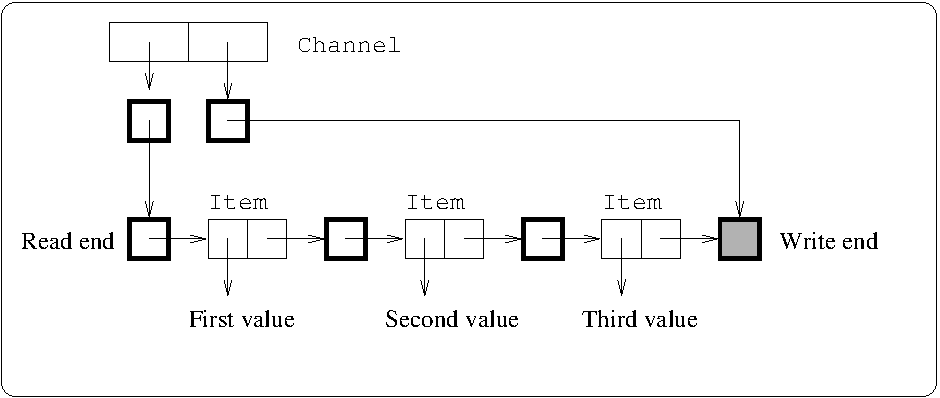
\includegraphics[scale=0.8]{channel.pdf}
\label{fig:channels}
\caption{Structure of the buffered channel implementation}
\end{figure}

\Subsubsection{channels}{Channels}

One of the strengths of @MVar@s is that they are a useful building
block out of which larger abstractions can be constructed.  Here we
will use @MVar@s to construct a unbounded buffered channel, supporting
the following basic interface:

\begin{haskell}
data Chan a

newChan   :: IO (Chan a)
readChan  :: Chan a -> IO a
writeChan :: Chan a -> a -> IO ()
\end{haskell}

\noindent This channel implementation first appeared in
\citet{jones96concurrent} (although the names were slightly
different), and is available in the Haskell module
@Control.Concurrent.Chan@.  The structure of the implementation is
represented diagrammatically in \figref{channels}, where each bold box
represents an @MVar@ and the lighter boxes are ordinary Haskell data
structures.  The current contents of the channel are represented as a
@Stream@, defined like this:

\begin{haskell}
type Stream a = MVar (Item a)
data Item a   = Item a (Stream a)
\end{haskell}

\noindent The end of the stream is represented by an empty @MVar@,
which we call the ``hole'', because it will be filled in when a new
element is added.  The channel itself is a pair of @MVar@s, one
pointing to the first element of the @Stream@ (the read position), and
the other pointing to the empty @MVar@ at the end (the write
position):

\begin{haskell}
data Chan a
 = Chan (MVar (Stream a))
        (MVar (Stream a))
\end{haskell}

To construct a new channel we must first create an empty @Stream@, which
is just a single empty @MVar@, and then the @Chan@ constructor with
@MVar@s for the read and write ends, both pointing to the empty
@Stream@:

\begin{haskell}
newChan :: IO (Chan a)
newChan = do
   hole  <- newEmptyMVar
   readVar  <- newMVar hole
   writeVar <- newMVar hole
   return (Chan readVar writeVar)
\end{haskell}

To add a new element to the channel we must make an @Item@ with a new
hole, fill in the current hole to point to the new item, and adjust
the write-end of the @Chan@ to point to the new hole:

\begin{haskell}
writeChan :: Chan a -> a -> IO ()
writeChan (Chan _ writeVar) val = do
  new_hole <- newEmptyMVar
  old_hole <- takeMVar writeVar
  putMVar writeVar new_hole
  putMVar old_hole (Item val new_hole)
\end{haskell}

To remove a value from the channel, we must follow the read end of the
@Chan@ to the first @MVar@ of the stream, take that @MVar@ to get the
@Item@, adjust the read end to point to the next @MVar@ in the stream,
and finally return the value stored in the @Item@:

\begin{numhaskell}
readChan :: Chan a -> IO a
readChan (Chan readVar _) = do
  stream <- takeMVar readVar
  Item val new <- takeMVar stream
  putMVar readVar new
  return val
\end{numhaskell}

\noindent Consider what happens if the channel is empty.  The first
@takeMVar@ (line 3) will succeed, but the second @takeMVar@ (line 4)
will find an empty hole, and so will block.  When another thread calls
@writeChan@, it will fill the hole, allowing the first thread to
complete its @takeMVar@, update the read end (line 5) and finally
return.

If multiple threads concurrently call @readChan@, the first one will
successfully call @takeMVar@ on the read end, but the subsequent
threads will all block at this point until the first thread completes
the operation and updates the read end.  If multiple threads call
@writeChan@, a similar thing happens: the write end of the @Chan@ is
the synchronisation point, only allowing one thread at a time to add
an item to the channel.  However, the read and write ends being
separate @MVar@s allows concurrent @readChan@ and @writeChan@
operations to proceed without interference.

This implementation allows a nice generalisation to \emph{multicast}
channels without changing the underlying structure.  The idea is to
add one more operation:

\begin{haskell}
dupChan :: Chan a -> IO (Chan a)
\end{haskell}

\noindent which creates a duplicate @Chan@ with the following
semantics:

\begin{itemize}
\item The new @Chan@ begins empty,
\item Subsequent writes to either @Chan@ are read from both; that is,
  reading an item from one @Chan@ does not remove it from the other.
\end{itemize}

The implementation is straightforward:

\begin{haskell}
dupChan :: Chan a -> IO (Chan a)
dupChan (Chan _ writeVar) = do
   hole       <- takeMVar writeVar
   putMVar writeVar hole
   newReadVar <- newMVar hole
   return (Chan newReadVar writeVar)
\end{haskell}

\noindent Both channels share a single write-end, but they have
independent read-ends.  The read end of the new channel is initialised
to point to the hole at the end of the current contents.

Sadly, this implementation of @dupChan@ does not work!  Can you see
the problem?  The definition of @dupChan@ itself is not at fault, but
combined with the definition of @readChan@ given earlier it does not
implement the required semantics.  The problem is that @readChan@ does
not replace the contents of a hole after having read it, so if
@readChan@ is called to read values from both the channel returned by
@dupChan@ and the original channel, the second call will block.  The fix is to change a
@takeMVar@ to @readMVar@ in the implementation of @readChan@:

\begin{numhaskell}
readChan :: Chan a -> IO a
readChan (Chan readVar _) = do
  stream <- takeMVar readVar
  Item val new <- readMVar stream -- modified
  putMVar readVar new
  return val
\end{numhaskell}

\noindent Line 4 returns the @Item@ back to the @Stream@, where it can
be read by any duplicate channels created by @dupChan@.

Before we leave the topic of channels, consider one more extension to
the interface that was described as an ``easy extension'' and left as
an exercise by \citet{jones96concurrent}:

\begin{haskell}
unGetChan :: Chan a -> a -> IO ()
\end{haskell}

\noindent the operation @unGetChan@ pushes a value back on the read
end of the channel.  Leaving aside for a moment the fact that the
interface does not allow the atomic combination of @readChan@ and
@unGetChan@ (which would appear to be an important use case), let us
consider how to implement @unGetChan@.  The straightforward
implementation is as follows:

\begin{numhaskell}
unGetChan :: Chan a -> a -> IO ()
unGetChan (Chan readVar _) val = do
   new_read_end <- newEmptyMVar
   read_end <- takeMVar readVar
   putMVar new_read_end (Item val read_end)
   putMVar readVar new_read_end
\end{numhaskell}

\noindent we create a new hole to place at the front of the @Stream@
(line 3), take the current read end (line 4) giving us the current
front of the stream, place a new @Item@ in the new hole (line 5), and
finally replace the read end with a pointer to our new item.

Simple testing will confirm that the implementation works.  However,
consider what happens when the channel is empty, there is already a
blocked @readChan@, and another thread calls @unGetChan@.  The desired
semantics is that @unGetChan@ succeeds, and @readChan@ should return
with the new element.  What actually happens in this case is deadlock:
the thread blocked in @readChan@ will be holding the read-end @MVar@,
and so @unGetChan@ will also block (line 4) trying to take the read
end.  As far as we know, there is no implementation of @unGetChan@
that has the desired semantics.

The lesson here is that programming larger structures with @MVar@ can
be much trickier than it appears.  As we shall see shortly, life gets
even more difficult when we consider exceptions.  Fortunately there is
a solution, that we will describe in \secref{stm}.

Despite the difficulties with scaling @MVar@s up to larger
abstractions, @MVar@s do have some nice properties, as we shall see in
the next section.

\Subsubsection{fairness}{Fairness}

Fairness is a well-studied and highly technical subject, which we do
not attempt to review here.  Nevertheless, we wish to highlight one
particularly important guarantee provided by @MVar@s with respect to
fairness:

\begin{quote}
No thread can be blocked indefinitely on an @MVar@ unless another
thread holds that @MVar@ indefinitely.
\end{quote}

In other words, if a thread $T$ is blocked in @takeMVar@, and there
are regular @putMVar@ operations on the same @MVar@, then it is
guaranteed that at some point thread $T$'s @takeMVar@ will return.  In
GHC this guarantee is implemented by keeping blocked threads in a FIFO
queue attached to the @MVar@, so eventually every thread in the queue
will get to complete its operation as long as there are other threads
performing regular @putMVar@ operations (an equivalent guarantee
applies to threads blocked in @putMVar@ when there are regular
@takeMVar@s).  Note that it is not enough to merely \emph{wake up} the
blocked thread, because another thread might run first and take
(respectively put) the @MVar@, causing the newly woken thread to go to
the back of the queue again, which would invalidate the fairness
guarantee.  The implementation must therefore atomically wake up the
blocked thread \emph{and} perform the blocked operation, which is
exactly what GHC does.

\paragraph{Fairness in practice}  Recall our example from \secref{forking}, where we had two threads,
one printing @A@s and the other printing @B@s, and the output was
often perfect alternation between the two: @ABABABABABABABAB@.  This
is an example of the fairness guarantee in practice.  The @stdout@
handle is represented by an @MVar@, so when both threads attempt to
call @takeMVar@ to operate on the handle, one of them wins and the
other becomes blocked.  When the winning thread completes its
operation and calls @putMVar@, the scheduler wakes up the blocked
thread \emph{and} completes its blocked @takeMVar@, so the original
winning thread will immediately block when it tries to re-acquire the
handle.  Hence this leads to perfect alternation between the two
threads.  The only way that the alternation pattern can be broken is if one
thread is pre-empted while it is not holding the @MVar@; indeed this
does happen from time to time, as we see the occasional long string of
a single letter in the output.

%  that this implementation does rely on some fairness in the
% scheduler too: the thread waiting to do the next @putMVar@ must not be
% indefinitely delayed, otherwise the fairness guarantee on @MVar@s
% fails.  At the current time GHC is using round-robin scheduling which
% satisfies this property.

A consequence of the fairness implementation is that, when multiple
threads are blocked, \emph{we only need to wake up a single thread}.
This single wakeup property is a particularly important performance
characteristic when a large number of threads are contending for a
single @MVar@.  As we shall see later, it is the fairness guarantee
together with the single-wakeup property which means that @MVar@s are
not completely subsumed by Software Transactional Memory.

\Subsection{async-exceptions}{Cancellation: Asynchronous Exceptions}

In an interactive application, it is often important for one thread to
be able to \emph{interrupt} the execution of another thread when some
particular condition occurs.  Some examples of this kind of behaviour
in practice include:

\begin{itemize}
\item In a web browser, the thread downloading the web page and the
  thread rendering the page need to be interrupted when the user
  presses the ``stop'' button.

\item A server application typically wants to give a client a set
  amount of time to issue a request before closing its connection, so
  as to avoid dormant connections using up resources.

\item An application in which a compute-intensive thread is working
  (say, rendering a visualisation of some data), and the input data
  changes due to some user input.
\end{itemize}

The crucial design decision in supporting cancellation is whether the
intended victim should have to poll for the cancellation condition,
or whether the thread is immediately cancelled in some way.  This is a
tradeoff:

\begin{enumerate}
\item If the thread has to poll, there is a danger that the programmer
  may forget to poll regularly enough, and the thread will become
  unresponsive, perhaps permanently so.  Unresponsive threads lead to
  hangs and deadlocks, which are particularly unpleasant from a
  user's perspective.
\item If cancellation happens asynchronously, critical sections that
  modify state need to be protected from cancellation, otherwise
  cancellation may occur mid-update leaving some data in an
  inconsistent state.
\end{enumerate}

In fact, the choice is really between doing only (1), or doing both
(1) and (2), because if (2) is the default, protecting a critical
section amounts to switching to polling behaviour for the duration of
the critical section.

In most imperative languages it is unthinkable for (2) to be the
default, because so much code is state-modifying.  Haskell has a
distinct advantage in this area, however: most code is purely
functional, so it can be safely aborted or suspended, and later
resumed, without affecting correctness.  Moreover our hand is
forced: purely functional code cannot by definition poll for the
cancellation condition, so it must be cancellable by default.

Therefore, fully-asynchronous cancellation is the only sensible
default in Haskell, and the design problem reduces to deciding how
cancellation appears to code in the @IO@ monad.

It makes sense for cancellation to behave like an exception, since
exceptions are already a fact of life in the @IO@ monad, and the usual
idioms for writing @IO@ monad code include exception handlers to
release resources and clean up in the event of an error.  For example,
to perform an operation that requires a temporary file, we would use
the @bracket@ combinator to ensure that the temporary file is always
removed, even if the operation raises an exception:

\begin{haskell}
  bracket (newTempFile "temp")
          (\file -> removeFile file)
          (\file -> ...)
\end{haskell}

\noindent where @bracket@ is defined thus:

\begin{haskell}
bracket :: IO a -> (a -> IO b) -> (a -> IO c) -> IO c
bracket before after during = do
  a <- before
  c <- during a `onException` after a
  after a
  return c
\end{haskell}

\noindent and @onException@ executes its first argument, and if an
exception is thrown, executes its second argument before re-throwing
the exception.

\begin{haskell}
onException :: IO a -> IO b -> IO a
\end{haskell}

We want exception handlers to run in the event of cancellation, so
cancellation should be an exception.  However, there's a fundamental
difference between the kind of exception thrown by @openFile@ when the
file does not exist, for example, and an exception that may arise
\emph{at any time} because the user pressed the ``stop'' button.  We
call the latter kind an \emph{asynchronous} exception, for obvious
reasons.  (We do not review the Haskell support for \emph{synchronous}
exceptions here; for that see the Haskell 2010 report
\cite{haskell2010} and the documentation for the @Control.Exception@
module).

To initiate an asynchronous exception, Haskell provides the @throwTo@
primitive which throws an exception from one thread to
another \cite{spj:asynch-exceptions}:

\begin{haskell}
throwTo :: Exception e => ThreadId -> e -> IO ()
\end{haskell}

\noindent the @Exception@ constraint requires that the exception value
being thrown is an instance of the @Exception@ class, which implements
a simple hierarchy \cite{extensible-exceptions}.  The @ThreadId@ is a
value previously returned by @forkIO@, and may refer to a thread in
any state: running, blocked, or finished (in the latter case,
@throwTo@ is a no-op).

To illustrate the use of @throwTo@, we now elaborate the earlier
example in which we downloaded several web pages concurrently, to
allow the user to hit @'q'@ at any time to stop the downloads.

First, we will extend our @Async@ mini-API to allow cancellation.  We
add one operation:

\begin{haskell}
cancel :: Async a -> IO ()
\end{haskell}

\noindent which cancels an existing @Async@.  If the operation has
already completed, @cancel@ has no effect.  The @wait@ operation
cannot just return the result of the @Async@ any more, since it may
have been cancelled.  Therefore, we extend @wait@ to return
@Either SomeException a@, containing either the exception raised during the
operation, or its result:

\begin{haskell}
wait :: Async a -> IO (Either SomeException a)
\end{haskell}

\noindent (@SomeException@ is the root of the exception hierarchy in Haskell.)
In order to implement the new interface, we need to extend the @Async@
type to include the @ThreadId@ of the child thread, and the @MVar@
holding the result must now hold @Either SomeException a@.

\begin{haskell}
data Async a = Async ThreadId (MVar (Either SomeException a))
\end{haskell}

\noindent Given this, the implementation of @cancel@ just throws an
exception to the thread:

\begin{haskell}
cancel :: Async a -> IO ()
cancel (Async t var) = throwTo t ThreadKilled
\end{haskell}

\noindent (@ThreadKilled@ is an exception provided by the Haskell exception
library and is typically used for cancelling threads in this way.)
The implementation of @wait@ is trivial.
The remaining piece of the implementation is the @async@ operation,
which must now include an exception handler to catch the exception and
store it in the @MVar@:

\begin{haskell}
async :: IO a -> IO (Async a)
async io = do
   m <- newEmptyMVar
   t <- forkIO $ (do r <- io; putMVar m (Right r))
                   `catch` \e -> putMVar m (Left e)
   return (Async t m)
\end{haskell}

Now, we can change the @main@ function of the example to support
cancelling the downloads:

\begin{numhaskell}
main = do
  as <- mapM (async.http) sites

  forkIO $ do
     hSetBuffering stdin NoBuffering
     forever $ do
        c <- getChar
        when (c == 'q') $ mapM_ cancel as

  rs <- mapM wait as
  printf "%d/%d finished\n" (length (rights rs)) (length rs)
\end{numhaskell}

\noindent Line 2 starts the downloads as before.  Lines 4--8 fork a
new thread that repeatedly reads characters from the standard input,
and if a @q@ is found, calls @cancel@ on all the @Async@s.  Line 10
waits for all the results (complete or cancelled), and line 11 emits a
summary with a count of how many of the operations completed without
being cancelled.  If we run the sample\footnote{full code is in the
  sample @geturlscancel.hs@} and hit @`q`@ fast enough, we see
something like this:

\begin{verbatim}
downloaded: http://www.google.com (14538 bytes, 0.17s)
downloaded: http://www.bing.com (24740 bytes, 0.22s)
q2/5 finished
\end{verbatim}

Note that this works even though the program is sitting atop a large
and complicated HTTP library that provides no direct support for
either cancellation or asynchronous I/O.  Haskell's support for
cancellation is modular in this respect: most library code needs to do
nothing to support it, although there are some simple and unintrusive
rules that need to be followed when dealing with state, as we shall
see in the next section.

\Subsubsection{mask}{Masking asynchronous exceptions}

As we mentioned earlier, the danger with fully asynchronous exceptions
is that one might fire while we are in the middle of updating some
shared state, leaving the data in an inconsistent state, and with a
high probability leading to mayhem later.

Hence, we certainly need a way to control the delivery of asynchronous
exceptions during critical sections.  But we must tread carefully: it
would be easy to provide the programmer with a way to turn off
asynchronous exception delivery temporarily, but such a facility is in
fact not what we really need.

Consider the following problem: a thread wishes to call @takeMVar@,
perform an operation depending on the value of the @MVar@, and finally
put the result of the operation in the @MVar@.  The code must be
responsive to asynchronous exceptions, but it should be safe: if an
asynchronous exception arrives after the @takeMVar@, but before the
final @putMVar@, the @MVar@ should not be left empty, instead the
original value should be replaced.

If we code up this problem using the facilities we already seen so
far, we might end up with something like this:

\begin{numhaskell}
problem m f = do
  a <- takeMVar m
  r <- f a `catch` \e -> do putMVar m a; throw e
  putMVar m r
\end{numhaskell}

\noindent There are at least two points where, if an asynchronous
exception strikes, the invariant will be violated.  If an exception
strikes between lines 2 and 3, or between lines 3 and 4, the @MVar@
will be left empty.  In fact, there is no way to shuffle around the
exception handlers to ensure the @MVar@ is always left full.  To fix
this problem, Haskell provides the @mask@
combinator\footnote{Historical note: the original presentation of
  asynchronous exceptions used a pair of combinators @block@ and
  @unblock@ here, but @mask@ was introduced in GHC 7.0.1 to replace
  them as it has a more modular behaviour.}:

\begin{haskell}
mask :: ((IO a -> IO a) -> IO b) -> IO b
\end{haskell}

\noindent The type looks a bit confusing, but it isn't
really\footnote{for simplicity here we are using a slightly less
  general version of @mask@ than the real one in the
  @Control.Exception@ library.}.  The @mask@ operation defers the
delivery of asynchronous exceptions for the duration of its argument,
and is used like this:

\begin{numhaskell}
problem m f = mask $ \restore -> do
  a <- takeMVar m
  r <- restore (f a) `catch` \e -> do putMVar m a; throw e
  putMVar m r
\end{numhaskell}

\noindent @mask@ is applied to a \emph{function}, that takes as its
argument a function @restore@, that can be used to restore the
delivery of asynchronous exceptions to its present state.  If we
imagine shading the entire argument to @mask@ except for the
expression @(f a)@, asynchronous exceptions cannot be raised in the
shaded portions.

This solves the problem that we had previously, since now an exception
can only be raised while @(f a)@ is working, and we have an exception
handler to catch any exceptions in that case.  But a new problem has
been introduced: @takeMVar@ might block for a long time, but it is
inside the @mask@ and so the thread will be unresponsive for that
time.  Furthermore there's no good reason to mask exceptions during
@takeMVar@; it would be safe for exceptions to be raised right up
until the point where @takeMVar@ returns.  Hence, this is exactly the
behaviour that Haskell defines for @takeMVar@: we designate a small
number of operations, including @takeMVar@, as \emph{interruptible}.
Interruptible operations may receive asynchronous exceptions even
inside @mask@.

What justifies this choice?  Think of @mask@ as ``switching to polling
mode'' for asynchronous exceptions.  Inside a @mask@, asynchronous
exceptions are no longer asynchronous, but they can still be raised by
certain operations.  In other words, asynchronous exceptions become
\emph{synchronous} inside @mask@.

All operations which may block indefinitely\footnote{except foreign
  calls, for technical reasons} are designated as interruptible.  This
turns out to be the ideal behaviour in many situations, as in
@problem@ above.

In fact, we can provide higher level combinators to insulate
programmers from the need to use @mask@ directly.  For example, the
function @problem@ above is generally useful when working with
@MVar@s, and is provided under the name @modifyMVar_@ in the
@Control.Concurrent.MVar@ library.

\Subsubsection{async-safety}{Asynchronous-exception safety}

All that is necessary for most code to be safe in the presence of
asynchronous exceptions is to use operations like @modifyMVar_@
instead of @takeMVar@ and @putMVar@ directly.  For example, consider
the buffered channels that we defined earlier.  As defined, the
operations are not asynchronous-exception-safe; for example,
@writeChan@ was defined like this:

\begin{numhaskell}
writeChan :: Chan a -> a -> IO ()
writeChan (Chan _ writeVar) val = do
  new_hole <- newEmptyMVar
  old_hole <- takeMVar writeVar
  putMVar writeVar new_hole
  putMVar old_hole (Item val new_hole)
\end{numhaskell}

\noindent there are several windows here where if an asynchronous
exception occurs, an @MVar@ will be left empty, and subsequent users
of the @Chan@ will deadlock.  To make it safe, we use @modifyMVar_@:

\begin{numhaskell}
writeChan (Chan _ writeVar) val = do
  new_hole <- newEmptyMVar
  modifyMVar_ writeVar $ \old_hole -> do
    putMVar old_hole (Item val new_hole)
    return new_hole
\end{numhaskell}

We saw a use of the @bracket@ function earlier; in fact, @bracket@ is
defined with @mask@ in order to make it asynchronous-exception-safe:

\begin{numhaskell}
bracket before after during =
  mask $ \restore -> do
    a <- before
    r <- restore (during a) `catch` \e -> after a; throw e
    _ <- after a
    return r
\end{numhaskell}

\Subsubsection{timeout}{Timeouts}

A good illustration of programming with asynchronous exceptions is to
write a function that can impose a time limit on a given action.  We
want to provide the timeout wrapper as a combinator of the following
type:

\begin{haskell}
timeout :: Integer -> IO a -> IO (Maybe a)
\end{haskell}

\noindent where @timeout @$t$@ @$m$ has the following behaviour:

\begin{enumerate}
\item @timeout @$t~m$ behaves exactly like @fmap Just @$m$ if $m$ returns a
  result or raises an exception (including an asynchronous exception),
  within $t$ microseconds.
\item otherwise, $m$ is sent an asynchronous exception of the form
  @Timeout @$u$.  @Timeout@ is a new datatype that we define, and $u$
  is a unique value of type @Unique@, distinguishing this particular
  instance of @timeout@ from any other.  The call to @timeout@ then
  returns @Nothing@.
\end{enumerate}

The implementation is not expected to implement real-time semantics,
so in practice the timeout will only be approximately $t$ microseconds.
Note that (1) requires that $m$ is executed in the context of the
current thread, since $m$ could call @myThreadId@, for example.  Also,
another thread throwing an exception to the current thread with
@throwTo@ will expect to interrupt $m$.

\begin{lstlisting}[float,label=lst:timeout,caption=implementation of \texttt{timeout},language=HaskellUlisses,style=numbers]
timeout n m
    | n <  0    = fmap Just m
    | n == 0    = return Nothing
    | otherwise = do
        pid <- myThreadId
        u <- newUnique
        let ex = Timeout u
        handleJust
           (\e -> if e == ex then Just () else Nothing)
           (\_ -> return Nothing)
           (bracket (forkIO $ do threadDelay n
                                 throwTo pid ex)
                    (\t -> throwTo t ThreadKilled)
                    (\_ -> fmap Just m))
\end{lstlisting}

The code for @timeout@ is shown in \lstref{timeout}; this
implementation was taken from the library @System.Timeout@ (with some
cosmetic changes for presentation here).  The implementation is tricky
to get right.  The basic idea is to fork a new thread that will wait
for $t$ microseconds and then call @throwTo@ to throw the @Timeout@
exception back to the original thread; that much seems straightforward
enough.  However, we must ensure that this thread cannot throw its
@Timeout@ exception after the call to @timeout@ has returned,
otherwise the @Timeout@ exception will leak out of the call, so
@timeout@ must kill the thread before returning.

Here is how the implementation works, line by line:

\begin{itemize}
\item[1--2] Handle the easy cases, where the timeout is
  negative or zero.
\item[5] find the @ThreadId@ of the current thread
\item[6--7] make a new @Timeout@ exception, by generating a unique value
  with @newUnique@
\item[8-14] @handleJust@ is an exception handler, with the following
  type:
\begin{haskell}
handleJust :: Exception e
           => (e -> Maybe b) -> (b -> IO a) -> IO a
           -> IO a
\end{haskell}
  Its first argument (line 9) selects which exceptions to catch: in
  this case, just the @Timeout@ exception we defined on line 7.  The
  second argument (line 10) is the exception handler, which in this
  case just returns @Nothing@, since timeout occurred.

  Lines 11--14 are the computation to run in the exception handler.
  @bracket@ (\secref{async-exceptions}) is used here in order to fork
  the child thread, and ensure that it is killed before returning.

  \begin{itemize}
    \item[11-12] fork the child thread.  In the child thread we wait
      for $n$ microseconds with @threadDelay@, and then throw the
      @Timeout@ exception to the parent thread with @throwTo@.
    \item [13] always kill the child thread before returning.
    \item [14] the body of @bracket@: run the computation @m@ passed
      in as the second argument to @timeout@, and wrap the result in
      @Just@.
  \end{itemize}
\end{itemize}

The reader is encouraged to verify that the implementation works by
thinking through the two cases: either @m@ completes and returns
@Just x@ at line 14, or, the child thread throws its exception while
@m@ is still working.

There is one tricky case to consider: what happens if \emph{both} the
child thread and the parent thread try to call @throwTo@ at the same
time (lines 12 and 13 respectively)?  Who wins?

The answer depends on the semantics of @throwTo@.  In order for this
implementation of @timeout@ to work properly, it must not be possible
for the call to @bracket@ at line 11 to return while the @Timeout@
exception can still be thrown, otherwise the exception can leak.
Hence, the call to @throwTo@ that kills the child thread at line 13
must be synchronous: once this call returns, the child thread cannot
throw its exception any more.  Indeed, this guarantee is provided by
the semantics of @throwTo@: a call to @throwTo@ only returns after the
exception has been raised in the target thread\footnote{Note: a
  different semantics was originally described in
  \citet{spj:asynch-exceptions}.}.  Hence, @throwTo@ may block if the
child thread is currently masking asynchronous exceptions with @mask@,
and because @throwTo@ may block, it is therefore \emph{interruptible}
and may itself receive asynchronous exceptions.

Returning to our ``who wins'' question above, the answer is ``exactly
one of them'', and that is precisely what we require to ensure the
correct behaviour of @timeout@.

\Subsubsection{async-reflections}{Asynchronous exceptions: reflections}

Abstractions like @timeout@ are certainly difficult to get right, but
fortunately they only have to be written once.  We find that in
practice dealing with asynchronous exceptions is fairly
straightforward, following a few simple rules:

\begin{itemize}
\item Use @bracket@ when acquiring resources that need to be released
  again.
\item Rather than @takeMVar@ and @putMVar@, use @modifyMVar_@ (and
  friends) which have built-in asynchronous exception safety.
\item If state handling starts getting complicated with multiple
  layers of exception handlers, then there are two approaches to
  simplifying things:
  \begin{itemize}
    \item Switching to polling mode with @mask@ can help manage
      complexity.  The GHC I/O library, for example, runs entirely
      inside @mask@.  Note that inside @mask@ it is important to
      remember that asynchronous exceptions can still arise out of
      interruptible operations; the documentation contains a list of
      operations that are guaranteed \emph{not} to be interruptible.
    \item Using Software Transactional Memory (STM) instead of @MVar@s
      or other state representations can sweep away all the complexity
      in one go.  We will describe STM in \secref{stm}.
  \end{itemize}
\end{itemize}

The rules are usually not onerous: remember this only applies to code
in the @IO@ monad, so the vast swathes of purely-functional library
code available for Haskell is all safe by construction.  We find that
most @IO@ monad code is straightforward to make safe, and if things
get complicated falling back to either @mask@ or STM is a satisfactory
solution.

In exchange for following the rules, however, Haskell's approach to
asynchronous exceptions confers many benefits.

\begin{itemize}
\item Many exceptional conditions map naturally onto asynchronous
  exceptions.  For example, stack overflow and user interrupt
  (e.g. control-C at the console) are mapped to asynchronous
  exceptions in Haskell.  Hence, control-C not only aborts the program
  but does so cleanly, running all the exception handlers.  Haskell
  programmers have to do nothing to enable this behaviour.

\item Constructs like @timeout@ always work, even with third-party
  library code.

\item Threads never just die in Haskell, it is guaranteed that a
  thread always gets a chance to clean up and run its exception
  handlers.
\end{itemize}

\Subsection{stm}{Software Transactional Memory}

Software Transactional Memory (STM) is a technique for simplifying
concurrent programming by allowing multiple state-changing operations
to be grouped together and performed as a single atomic operation.
Strictly speaking, ``Software Transactional Memory'' is an
implementation technique, whereas the language construct we are
interested in is ``atomic blocks''.  Unfortunately the former term has
stuck, and so the language-level facility is called STM.

STM solves a number of problems that arise with conventional
concurrency abstractions, that we describe here through a series of
examples.  For reference throughout the following section, the types
and operations of the STM interface are collected in
\lstref{stm}.

\begin{lstlisting}[float,label=lst:stm,caption=the interface
    provided by \texttt{Control.Concurrent.STM},language=HaskellUlisses,style=numbers]
data STM a -- abstract
instance Monad STM -- amongst other things

atomically :: STM a -> IO a

data TVar a -- abstract
newTVar   :: a -> STM (TVar a)
readTVar  :: TVar a -> STM a
writeTVar :: TVar a -> a -> STM ()

retry     :: STM a
orElse    :: STM a -> STM a -> STM a

throwSTM  :: Exception e => e -> STM a
catchSTM  :: Exception e => STM a -> (e -> STM a) -> STM a
\end{lstlisting}


Imagine the following scenario: a window manager that manages multiple
desktops.  The user may move windows from one desktop to another,
while at the same time, a program may request that its own window
moves from its current desktop to another desktop.  The window manager
uses multiple threads: one to listen for input from the user, one for
each existing window to listen for requests from those programs, and
one thread that renders the display to the user.

How should the program represent the state of the display?  One option
is to put it all in a single @MVar@:

\begin{haskell}
type Display = MVar (Map Desktop (Set Window))
\end{haskell}

\noindent and this would work, but the @MVar@ is a single point of
contention.  For example, the rendering thread, which only needs to
look at the currently displayed desktop, could be blocked by a window
on another desktop moving itself.

So perhaps we can try to allow more concurrency by having a separate
@MVar@ for each desktop:

\begin{haskell}
type Display = Map Desktop (MVar (Set Window))
\end{haskell}

\noindent unfortunately this approach quickly runs into problems.
Consider an operation to move a window from one desktop to another:

\begin{haskell}
moveWindow :: Display -> Window -> Desktop -> Desktop -> IO ()
moveWindow disp win a b = do
  wa <- takeMVar ma
  wb <- takeMVar mb
  putMVar ma (Set.delete win wa)
  putMVar mb (Set.insert win wb)
 where
  ma = fromJust (Map.lookup disp a)
  mb = fromJust (Map.lookup disp b)
\end{haskell}

\noindent Note that we must take both @MVar@s before we can put the
results: otherwise another thread could potentially observe the
display in a state in which the window we are moving does not exist.
But this raises a problem: what if there is concurrent call to
@moveWindow@ trying to move a window in the opposite direction?  Both
calls would succeed at the first @takeMVar@, but block on the second,
and the result is a deadlock.  This is an instance of the classic
Dining Philosophers problem. % \cite{}.

One solution is to impose an ordering on the @MVar@s, and require that
all agents take @MVar@s in the correct order and release them in
the opposite order.  That is inconvenient and error-prone though, and
furthermore we have to extend our ordering to any other state that we
might need to access concurrently.  Large systems with many
locks (e.g. Operating Systems) are often plagued by this problem, and
managing the complexity requires building elaborate infrastructure to
detect ordering violations.

Transactional memory provides a way to avoid this deadlock problem
without imposing a requirement for ordering on the programmer.  To
solve the problem using STM, we replace @MVar@ with @TVar@:

\begin{haskell}
type Display = Map Desktop (TVar (Set Window))
\end{haskell}

\noindent @TVar@ stands for ``transactional variable'', and it is a
mutable variable that can only be read or written within a
transaction.  To implement @moveWindow@, we simply perform the
necessary operations on @TVar@s in the STM monad, and wrap the whole
sequence in @atomically@:

\begin{haskell}
moveWindow :: Display -> Window -> Desktop -> Desktop -> IO ()
moveWindow disp win a b = atomically $ do
  wa <- readTVar ma
  wb <- readTVar mb
  writeTVar ma (Set.delete win wa)
  writeTVar mb (Set.insert win wb)
 where
  ma = fromJust (Map.lookup a disp)
  mb = fromJust (Map.lookup b disp)
\end{haskell}

\noindent The code is almost identical to the @MVar@ version, but the
behaviour is quite different: the sequence of operations inside
@atomically@ happens indivisibly as far as the rest of the program is
concerned.  No other thread can observe an intermediate state; the
operation has either completed, or it has not started yet.  What's
more, there is no requirement that we read both @TVar@s before we
write them, this would be fine too:

\begin{haskell}
moveWindow :: Display -> Window -> Desktop -> Desktop -> IO ()
moveWindow disp win a b = atomically $ do
  wa <- readTVar ma
  writeTVar ma (Set.delete win wa)
  wb <- readTVar mb
  writeTVar mb (Set.insert win wb)
 where
  ma = fromJust (Map.lookup disp a)
  mb = fromJust (Map.lookup disp b)
\end{haskell}

\noindent So STM is far less error-prone here.  The approach also
scales to any number of @TVar@s, so we could easily write an operation
that moves the windows from all other desktops to the current desktop,
for example.

Now suppose that we want to swap two windows, moving window W from
desktop A to B, and simultaneously V from B to A.  With the @MVar@
representation we would have to write a special-purpose operation to
do this, because it has to take the @MVar@s for A and B (in the right
order), and then put both @MVar@s back with the new contents.  With
STM, however, we can express this much more neatly as a composition.
First we need to expose a version of @moveWindow@ without the
@atomically@ wrapper:

\begin{haskell}
moveWindowSTM :: Display -> Window -> Desktop -> Desktop
              -> STM ()
moveWindowSTM disp win a b = do ...
\end{haskell}

\noindent and then we can define @swapWindows@ by composing two
@moveWindowSTM@ calls:

\begin{haskell}
swapWindows :: Display
            -> Window -> Desktop
            -> Window -> Desktop
            -> IO ()
swapWindows disp w a v b = atomically $ do
  moveWindowSTM disp w a b
  moveWindowSTM disp v b a
\end{haskell}

\noindent This demonstrates the \emph{composability} of STM
operations: any operation of type @STM a@ can be composed with others
to form a larger atomic transaction.  For this reason, @STM@
operations are usually provided without the @atomically@ wrapper, so
that clients can compose them as necessary, before finally wrapping
the entire operation in @atomically@.

So far we have covered the basic facilities of STM, and shown that STM
can be used to make atomicity scale in a composable way.  STM confers
a qualitative improvement in expressibility and robustness when
writing concurrent programs.  The benefits of STM in Haskell go
further, however: in the following sections we show how STM can be
used to make blocking abstractions compose, and how STM can be used to
manage complexity in the presence of failure and interruption.

\Subsubsection{stm-blockng}{Blocking}

An important part of concurrent programming is dealing with
\emph{blocking}; when we need to wait for some condition to be true,
or to acquire a particular resource.  STM provides an ingenious way to
do this, with a single operation:

\begin{haskell}
retry :: STM a
\end{haskell}

\noindent the meaning of @retry@ is simply ``run the current
transaction again''.  That seems bizarre - why would we want to run
the current transaction again?  Well, for one thing, the contents of
some @TVar@s that we have read may have been changed by another
thread, so re-running the transaction may yield different results.
Indeed, there's no point re-running the transaction \emph{unless} it
is possible that something different might happen, and the runtime
system knows this, so @retry@ waits until a @TVar@ that was read in
the current transaction has been written to, and then triggers a
re-run of the current transaction.  Until that happens, the current
thread is blocked.

\ToDo{perhaps rearrange the text here, at least one reader was
  confused because the discussion of ``not busy waiting'' occurs
  before the concrete example.}

As a concrete example, we can use @retry@ to implement the rendering
thread in our window-manager example.  The behaviour we want is this:

\begin{itemize}
\item One desktop is designated as having the \emph{focus}.  The
  focussed desktop is the one displayed by the rendering thread.
\item The user may request that the focus be changed at any time.
\item Windows may move around and appear or disappear of their own
  accord, and the rendering thread must update its display
  accordingly.
\end{itemize}

We are supplied with a function @render@ which handles the business of
rendering windows on the display.  It should be called whenever the
window layout changes\footnote{we are assuming that the actual window contents
are rendered via some separate means, e.g. compositing}:

\begin{haskell}
render :: Set Window -> IO ()
\end{haskell}

The currently focussed desktop is a piece of state that is shared by
the rendering thread and some other thread that handles user input.
Therefore we represent that by a @TVar@:

\begin{haskell}
type UserFocus = TVar Desktop
\end{haskell}

Next, we define an auxiliary function @getWindows@ that takes the
@Display@ and the @UserFocus@, and returns the set of windows to render,
in the @STM@ monad.  The implementation is straightforward: read the
current focus, and look up the contents of the appropriate desktop in
the @Display@:

\begin{haskell}
getWindows :: Display -> UserFocus -> STM (Set Window)
getWindows disp focus = do
  desktop <- readTVar focus
  readTVar (fromJust (Map.lookup desktop disp))
\end{haskell}

Finally, we can implement the rendering thread.  The general plan is
to repeatedly read the current state with @getWindows@ and call
@render@ to render it, but use @retry@ to avoid calling @render@ when
nothing has changed.  Here is the code:

\begin{numhaskell}
renderThread :: Display -> UserFocus -> IO ()
renderThread disp focus = do
  wins <- atomically $ getWindows disp focus
  loop wins
 where
  loop wins = do
    render wins
    next <- atomically $ do
               wins' <- getWindows disp focus
               if (wins == wins')
                   then retry
                   else return wins'
    loop next
\end{numhaskell}

\noindent First we read the current set of windows to display (line 3)
and use this as the initial value for the @loop@ (line 4).  Lines 6-13
implement the loop.  Each iteration calls @render@ to display the
current state (line 7), and then enters a transaction to read the next
state.  Inside the transaction we read the current state (line 9), and
compare it to the state we just rendered (line 10); if the states are
the same, there is no need to do anything, so we call @retry@.  If the
states are different, then we return the new state, and the loop
iterates with the new state (line 13).

The effect of the @retry@ is precisely what we need: it waits until
the value read by @getWindows@ could possibly be different, because
another thread has successfully completed a transaction that writes to
one of the @TVar@s that is read by @getWindows@.  That encompasses
both changes to the @focus@ (because the user switched to a different
desktop), and changes to the contents of the current desktop (because
a window moved, appeared, or disappeared).  Furthermore, changes to
other desktops can take place without the rendering thread being woken
up.

If it weren't for STM's @retry@ operation, we would have to implement
this complex logic ourselves, including implementing the signals
between threads that modify the state and the rendering thread.  This
is anti-modular, because operations that modify the state have to know
about the observers that need to act on changes.  Furthermore, it
gives rise to a common source of concurrency bugs: \emph{lost
  wakeups}.  If we forgot to signal the rendering thread, then the
display would not be updated.  In this case the effects are somewhat
benign, but in a more complex scenario lost wakeups often lead to
deadlocks, because the woken thread was supposed to complete some
operation on which other threads are waiting.

\Subsubsection{tchan}{Implementing channels with STM}

As a second concrete example, we shall implement the @Chan@ type from
\secref{channels} using STM.  We shall see that using STM to implement
@Chan@ is rather less tricky than using @MVar@s, and furthermore we
are able to add some more complex operations that were hard or
impossible using @MVar@s.

The STM version of @Chan@ is called @TChan@\footnote{the implementation
  is available in the module @Control.Concurrent.STM.TChan@ from the
  @stm@ package.}, and the interface we wish to implement is as
follows:

\begin{lstlisting}[float,label=lst:tchan,caption=implementation of \texttt{TChan},language=HaskellUlisses,style=numbers]
data TChan a = TChan (TVar (TVarList a))
                     (TVar (TVarList a))

type TVarList a = TVar (TList a)
data TList a = TNil | TCons a (TVarList a)

newTChan :: STM (TChan a)
newTChan = do
  hole <- newTVar TNil
  read <- newTVar hole
  write <- newTVar hole
  return (TChan read write)

readTChan :: TChan a -> STM a
readTChan (TChan readVar _) = do
  listhead <- readTVar readVar
  head <- readTVar listhead
  case head of
    TNil -> retry
    TCons val tail -> do
        writeTVar readVar tail
        return val

writeTChan :: TChan a -> a -> STM ()
writeTChan (TChan _ writeVar) a = do
  new_listend <- newTVar TNil
  listend <- readTVar writeVar
  writeTVar writeVar new_listend
  writeTVar listend (TCons a new_listend)
\end{lstlisting}

\begin{haskell}
data TChan a

newTChan   :: STM (TChan a)
writeTChan :: TChan a -> a -> STM ()
readTChan  :: TChan a -> STM a
\end{haskell}

\noindent that is, exactly the same as @Chan@, except that we renamed
@Chan@ to @TChan@.  The full code for the implementation is given in
\lstref{tchan}.  The implementation is similar in structure to the
@MVar@ version in \secref{channels}, so we do not describe it line by
line, however we shall point out a few important details:

\begin{itemize}
\item All the operations are in the @STM@ monad, so to use them they
  need to be wrapped in @atomically@ (but they can also be composed,
  more about that later).
\item Blocking in @readTChan@ is implemented by the call to @retry@
  (line 19).
\item Nowhere did we have to worry about what happens when a read
  executes concurrently with a write, because all the operations are
  atomic.
\end{itemize}

Something worth noting, although this is not a direct result of STM,
is that the straightforward implementation of @dupChan@ does not
suffer from the problem that we had in \secref{channels}, because
@readTChan@ does not remove elements from the list.

We now describe three distinct benefits of the STM implementation
compared to using @MVar@s.

\paragraph{More operations are possible.} In \secref{channels} we
mentioned the operation @unGetChan@, which could not be implemented
with the desired semantics using @MVar@s.  Here is its implementation
with STM:

\begin{haskell}
unGetTChan :: TChan a -> a -> STM ()
unGetTChan (TChan read _write) a = do
   listhead <- readTVar read
   newhead <- newTVar (TCons a listhead)
   writeTVar read newhead
\end{haskell}

\noindent The obvious implementation does the right thing here.  Other
operations that were not possible with @MVar@s are straightforward
with STM, for example @isEmptyTChan@, the @MVar@ version of which
suffers from the same problem as @unGetChan@:

\begin{haskell}
isEmptyTChan :: TChan a -> STM Bool
isEmptyTChan (TChan read _write) = do
  listhead <- readTVar read
  head <- readTVar listhead
  case head of
    TNil -> return True
    TCons _ _ -> return False
\end{haskell}

\paragraph{Composition of blocking operations.}  Suppose we wish to
implement an operation @readEitherTChan@ that can read an element from
either of two channels.  If both channels are empty it blocks; if one
channel is non-empty it reads the value from that channel, and if both
channels are non-empty it is allowed to choose which channel to read
from.  Its type is

\begin{haskell}
readEitherTChan :: TChan a -> TChan b -> STM (Either a b)
\end{haskell}

\noindent We cannot implement this function with the operations
introduced so far, but STM provides one more crucial operation that
allows blocking transactions to be composed.  The operation is
@orElse@:

\begin{haskell}
orElse :: STM a -> STM a -> STM a
\end{haskell}

\noindent The operation @orElse a b@ has the following behaviour:

\begin{itemize}
\item First @a@ is executed.  If @a@ returns a result, then that
  result is immediately returned by the @orElse@ call.
\item If @a@ instead called @retry@, then \emph{@a@'s effects are
  discarded}, and @b@ is executed instead.
\end{itemize}

We can use @orElse@ to compose blocking operations atomically.
Returning to our example, @readEitherTChan@ could be implemented as
follows:

\begin{haskell}
readEitherTChan :: TChan a -> TChan b -> STM (Either a b)
readEitherTChan a b =
  fmap Left (readTChan a)
    `orElse`
  fmap Right (readTChan b)
\end{haskell}

\noindent This is a straightforward composition of the two @readTChan@ calls,
the only complication is arranging to tag the result with either
@Left@ or @Right@ depending on which branch succeeds.

In the @MVar@ implementation of @Chan@ there is no way to implement
the operation @readEitherChan@ without elaborating the representation of @Chan@ to
support the synchronisation protocol that would be required (more
discussion on implementing choice with @MVar@s can be found in
\citet{jones96concurrent}).

One thing to note is that @orElse@ is left-biased; if both @TChan@s
are non-empty, then @readEitherChan@ will always return an element
from the first one.  Whether this is problematic or not depends on the
application: something to be aware of is that the left-biased nature
of @orElse@ can have implications for fairness in some situations.

\paragraph{Asynchronous exception safety.} Up until now we have said
nothing about how exceptions in STM behave.  The @STM@ monad supports
exceptions much like the @IO@ monad, with two operations:

\begin{haskell}
throwSTM  :: Exception e => e -> STM a
catchSTM  :: Exception e => STM a -> (e -> STM a) -> STM a
\end{haskell}

\noindent @throwSTM@ throws an exception, and @catchSTM@ catches
exceptions and invokes a handler, just like @catch@ in the @IO@ monad.
However, exceptions in STM are different in one vital way:

\begin{itemize}
\item In @catchSTM m h@, if @m@ raises an exception, then \emph{all of
  its effects are discarded}, and then the handler @h@ is invoked.  As
  a degenerate case, if there is no enclosing @catchSTM@ at all, then
  all of the effects of the transaction are discarded and the
  exception is propagated out of @atomically@.
\end{itemize}

\noindent This behaviour of @catchSTM@ was introduced in a subsequent
amendment of \citet{stm}; the original behaviour in which effects were
not discarded being generally regarded as much less useful.  An
example helps to demonstrate the motivation:

\begin{haskell}
readCheck :: TChan a -> STM a
readCheck chan = do
  a <- readTChan chan
  checkValue a
\end{haskell}

\noindent @checkValue@ imposes some extra constraints on the value
read from the channel.  However, suppose @checkValue@ raises an
exception (perhaps accidentally, e.g. divide-by-zero).  We would
prefer it if the @readTChan@ had not happened, since an element of the
channel would be lost.  Furthermore, we would like @readCheck@ to have
this behaviour regardless of whether there is an enclosing exception
handler or not.  Hence @catchSTM@ discards the effects of its first
argument in the event of an exception.

The discarding-effects behaviour is even more useful in the case of
\emph{asynchronous} exceptions.  If an asynchronous exception occurs
during an STM transaction, the entire transaction is aborted (unless
the exception is caught and handled, but handling asynchronous
exceptions in STM is not something we typically want to do).  So in
most cases, asynchronous exception safety in STM consists of doing
\emph{absolutely nothing at all}.  There are no locks to replace, so
no need for exception handlers or @bracket@, and no need to worry
about which critical sections to protect with @mask@.

The implementation of @TChan@ given earlier is entirely safe with
respect to asynchronous exceptions as it stands, and moreover any
compositions of these operations are also safe.

STM provides a nice way to write code that is automatically safe with
respect to asynchronous exceptions, so it can be useful even for state
that is not shared between threads.  The only catch is that we have to
use STM consistently for all our state, but having made that leap,
asynchronous exception safety comes for free.

\Subsubsection{stm-cost}{Performance}

As with most abstractions, STM has a runtime cost.  If we understand
the cost model, then we can avoid writing code that hits the bad
cases.  So in this section we give an informal description of the
implementation of STM (at least in GHC), with enough detail that the
reader can understand the cost model.

An STM transaction works by accumulating a \emph{log} of @readTVar@
and @writeTVar@ operations that have happened so far during the
transaction.  The log is used in three ways:

\begin{itemize}
\item By storing @writeTVar@ operations in the log rather than
  applying them to main memory immediately, discarding the effects of
  a transaction is easy; we just throw away the log.  Hence, aborting
  a transaction has a fixed small cost.

\item Each @readTVar@ must traverse the log to check whether the
  @TVar@ was written by an earlier @writeTVar@.  Hence, @readTVar@ is
  an $O(n)$ operation in the length of the log.

\item Because the log contains a record of all the @readTVar@
  operations, it can be used to discover the full set of @TVar@s read
  during the transaction, which we need to know in order to implement
  @retry@.
\end{itemize}

When a transaction reaches the end, the STM implementation compares
the log against the contents of memory using a two-phase locking
protocol (details in \citet{stm}).  If the current contents of memory
matches the values read by @readTVar@, the effects of the transaction
are \emph{committed} to memory atomically, and if not, the log is
discarded and the transaction runs again from the beginning.  The STM
implementation in GHC does not use global locks; only the @TVar@s
involved in the transaction are locked during commit, so transactions
operating on disjoint sets of @TVar@s can proceed without
interference.

The general rule of thumb when using STM is never to read an unbounded
number of @TVar@s in a single transaction, because the $O(n)$
performance of @readTVar@ then gives $O(n^2)$ for the whole
transaction.  Furthermore, long transactions are much more likely to
fail to commit, because another transaction will probably have
modified one or more of the same @TVar@s in the meantime, so there is
a high probability of re-execution.

It is possible that a future STM implementation may use a different
data structure to store the log, reducing the @readTVar@ overhead to
$O(\mbox{log}~n)$ or better (on average), but the likelihood that a
long transaction will fail to commit would still be an issue.  To
avoid that problem intelligent contention-management is required,
which is an area of active research.

\ToDo{describe the implementation of retry}

\Subsubsection{stm-summary}{Summary}

To summarise, STM provides several benefits for concurrent
programming:

\begin{itemize}
\item \textbf{Composable atomicity}.  We may construct arbitrarily large atomic
  operations on shared state, which can simplify the implementation of
  concurrent data structures with fine-grained locking.
\item \textbf{Composable blocking}.  We can build operations that make
  a choice between multiple blocking operations; something which is
  very difficult with @MVar@s and other low-level concurrency
  abstractions.
\item \textbf{Robustness in the presence of failure and cancellation}.
  A transaction in progress is aborted if an exception occurs, so STM
  makes it easy to maintain invariants on state in the presence of
  exceptions.
\end{itemize}

\Subsubsection{stm-further}{Further reading}

To find out more about STM in Haskell:

\begin{itemize}
\item \citet{stm}, the original paper describing the design of
  Haskell's STM interface (be sure to get the revised
  version\footnote{\url{http://research.microsoft.com/people/simonpj/}}
  which has the modified semantics for exceptions).
\item ``Beautiful Concurrency'' a chapter in \citet{beautiful-code}.
\end{itemize}

\Subsection{conc-ffi}{Concurrency and the Foreign Function Interface}

Haskell has a \emph{foreign function interface} (FFI) that allows
Haskell code to call, and be called by, foreign language code
(primarily C) \cite{haskell2010}.  Foreign languages also have their
own threading models --- in C there is POSIX or Win32 threads, for
example --- so we need to specify how Concurrent Haskell interacts
with the threading models of foreign code.

The details of the design can be found in \citet{conc-ffi}, in the
following sections we summarise the behaviour the Haskell programmer
can expect.

All of the following assumes that GHC's @-threaded@ option is in use.
Without @-threaded@, the Haskell process uses a single OS thread only,
and multi-threaded foreign calls are not supported.

\Subsubsection{conc-ffi-outcall}{Threads and foreign out-calls}

An out-call is a call made from Haskell to a foreign language.  At the
present time the FFI supports only calls to C, so that's all we
describe here.  In the following we refer to threads in C (i.e. POSIX
or Win32 threads) as ``OS threads'' to distinguish them from Haskell
threads.

As an example, consider making the POSIX C function @read()@ callable
from Haskell:

\begin{haskell}
foreign import ccall "read"
   c_read :: CInt      -- file descriptor
          -> Ptr Word8 -- buffer for data
          -> CSize     -- size of buffer
          -> CSSize    -- bytes read, or -1 on error
\end{haskell}

\noindent This declares a Haskell function @c_read@ that can be used
to call the C function @read()@.  Full details on the syntax of
@foreign@ declarations and the relationship between C and Haskell
types can be found in the Haskell report \cite{haskell2010}.

Just as Haskell threads run concurrently with each other, when a
Haskell thread makes a foreign call, that foreign call runs
concurrently with the other Haskell threads, and indeed with any other
active foreign calls.  Clearly the only way that two C calls can be
running concurrently is if they are running in two separate OS
threads, so that is exactly what happens: if several Haskell threads
call @c_read@ and they all block waiting for data to be read, there
will be one OS thread per call blocked in @read()@.

This has to work despite the fact that Haskell threads are not
normally mapped one-to-one with OS threads; as we mentioned earlier
(\secref{forking}), in GHC, Haskell threads are lightweight and
managed in user-space by the runtime system.  So to handle concurrent
foreign calls, the runtime system has to create more OS threads, and
in fact it does this on demand.  When a Haskell thread makes a foreign
call, another OS thread is created (if necessary), and the
responsibility for running the remaining Haskell threads is handed
over to the new OS thread, meanwhile the current OS thread makes the
foreign call.

The implication of this design is that a foreign call may be executed
in \emph{any} OS thread, and subsequent calls may even be executed in
different OS threads. In most cases this isn't important, but
sometimes it is: some foreign code must be called by a \emph{particular}
OS thread.  There are two instances of this requirement:

\begin{itemize}
\item Libraries that only allow one OS thread to use their API.  GUI
  libraries often fall into this category: not only must the library
  be called by only one OS thread, it must often be one
  \emph{particular} thread (e.g. the main thread).  The Win32 GUI APIs
  are an example of this.

\item APIs that use internal thread-local state.  The best-known
  example of this is OpenGL, which supports multi-threaded use, but
  stores state between API calls in thread-local storage.  Hence,
  subsequent calls must be made in the same OS thread, otherwise the
  later call will see the wrong state.
\end{itemize}

For this reason, the concept of \emph{bound threads} was introduced.
A bound thread is a Haskell thread/OS thread pair, such that foreign
calls made by the Haskell thread always take place in the associated
OS thread.  A bound thread is created by @forkOS@:

\begin{haskell}
forkOS :: IO () -> IO ThreadId
\end{haskell}

\noindent Care should be taken when calling @forkOS@: it creates a
complete new OS thread, so it can be quite expensive.

\Subsubsection{conc-ffi-incall}{Threads and foreign in-calls}

In-calls are calls to Haskell functions that have been exposed to
foreign code using @foreign export@.  For example, if we have a
function @f@ of type @Int -> IO Int@, we could expose it like this:

\begin{haskell}
foreign export ccall "f" f :: Int -> IO Int
\end{haskell}

\noindent This would create a C function with the following signature:

\begin{haskell}
HsInt f(HsInt);
\end{haskell}

\noindent here @HsInt@ is the C type corresponding to Haskell's @Int@
type.

In a multi-threaded program, it is entirely possible that @f@ might be
called by multiple OS threads concurrently.  The GHC runtime system
supports this (at least with @-threaded@), with the following
behaviour: each call becomes a new \emph{bound thread}.  That is, a
new Haskell thread is created for each call, and the Haskell thread is
bound to the OS thread that made the call.  Hence, any further
out-calls made by the Haskell thread will take place in the same OS
thread that made the original in-call.  This turns out to be important
for dealing with GUI callbacks: the GUI wants to run in the main OS
thread only, so when it makes a callback into Haskell, we need to
ensure that GUI calls made by the callback happen in the same OS
thread that invoked the callback.

\Subsubsection{conc-ffi-further}{Further reading}

\begin{itemize}
\item The full specification of the Foreign Function Interface (FFI)
  can be found in the Haskell 2010 report \cite{haskell2010};
\item GHC's extensions to the FFI can be found in the GHC User's
  Guide\footnote{\url{http://www.haskell.org/ghc/docs/latest/html/users_guide/}};
\item Functions for dealing with bound threads can be found in the
  documentation for the @Control.Concurrent@ module.
\end{itemize}

\Subsection{conc-io}{High-speed concurrent server applications}

Server-type applications that communicate with many clients
simultaneously demand both a high degree of concurrency and high
performance from the I/O subsystem.  A good web server should be able
to handle hundreds of thousands of concurrent connections, and service
tens of thousands of requests per second.

Ideally, we would like to write these kinds of applications using
threads.  A thread is the right abstraction: it allows the developer
to focus on programming the interaction with a single client, and then
to lift this interaction to multiple clients by simply forking many
instances of the single-client interaction in separate threads.  To
illustrate this idea we will describe a simple network
server\footnote{the full code can be found in sample @server.hs@},
with the following behaviour:

\begin{itemize}
\item The server accepts connections from clients on port 44444.
\item If a client sends an integer $n$, the service responds with the value of
  $2n$
\item If a client sends the string @"end"@, the server closes the
  connection.
\end{itemize}

First, we program the interaction with a single client.  The function
@talk@ defined below takes a @Handle@ for communicating with the
client.  The @Handle@ is typically bound to a network socket, so data
sent by the client can be read from the @Handle@, and data written to
the @Handle@ will be sent to the client.

\begin{numhaskell}
talk :: Handle -> IO ()
talk h = do
  hSetBuffering h LineBuffering
  loop
 where
  loop = do
    line <- hGetLine h
    if line == "end"
       then hPutStrLn h ("Thank you for using the " ++
                         "Haskell doubling service.")
       else do hPutStrLn h (show (2 * (read line :: Integer)))
               loop
\end{numhaskell}

\noindent Line 3 sets the buffering mode for the @Handle@ to
line-buffering; if we don't do that then output sent to the @Handle@
will be buffered up by the I/O layer until there is a full block
(which is more efficient for large transfers, but not useful for
interactive applications).  Then we enter a loop to respond to
requests from the client.  Each iteration of the loop reads a new line
of text (line 7), and then checks whether the client sent @"end"@.  If
so, we emit a polite message and return (line 8).  If not, we attempt
to interpret the line as an integer and to write the value obtained by
doubling it.  Finally we call @loop@ again to read the next request.

Having dealt with the interaction with a single client, we can now
make this into a multi-client server using concurrency.  The @main@
function for our server is as follows:

\begin{numhaskell}
main = do
  s <- listenOn (PortNumber 44444)
  forever $ do
    (h,host,_) <- accept s
    printf "new client: %s\n" host
    forkIO (talk h `finally` hClose h)
\end{numhaskell}

\noindent On line 2 we create a network socket to listen on port
44444, and then we enter a loop to accept connections from clients
(line 3).  Line 4 accepts a new client connection: @accept@ blocks
until a connection request from a client arrives, and then returns a
@Handle@ for communicating with the client (here bound to @h@) and
some information about the client (here we bind @host@ to the client's
hostname).  Line 5 reports the new connection, and on line 6 we call
@forkIO@ to create a new thread to handle the request.  A little
explanation is needed for the expression passed to @forkIO@:

\begin{haskell}
   talk h `finally` hClose h
\end{haskell}

\noindent @talk@ is the single-client interaction that we defined
above.  The function @finally@ is a standard exception-handling
combinator.  It is rather like a specialised version
of @bracket@, and has the following type

\begin{haskell}
finally :: IO a -> IO b -> IO a
\end{haskell}

\noindent with the behaviour that @a `finally` b@ behaves exactly like
@a@, except that @b@ is always performed after @a@ returns or throws
an exception.  Here we are using @finally@ to ensure that the @Handle@
for communicating with the client is always closed, even if @talk@
throws an exception.  If we didn't do this, the @Handle@ would
eventually be garbage collected, but in the meantime it would consume
resources which might lead to the program failing due to lack of file
descriptors.  It is always a good idea to close @Handle@s when you're
finished with them.

Having forked a thread to handle this client, the main thread then
goes back to accepting more connections.  All the active client
connections and the main thread run concurrently with each other, so
the fact that the server is handling multiple clients will be
invisible to any individual client (unless the server becomes
overloaded).

So, making our concurrent server was simple - we did not have to
change the single-client code at all, and the code to lift it to a
concurrent server was only a handful of lines.  We can verify that it
works: in one window we start the server

\begin{verbatim}
$ ./server
\end{verbatim}

\noindent in another window we start a client, and try a single
request\footnote{@nc@ is the netcat program, which is useful for simple network
  interaction}:

\begin{verbatim}
$ nc localhost 44444
22
44
\end{verbatim}

\noindent Next we leave this client running, and start another client:

\begin{verbatim}
$ ghc -e 'mapM_ print [1..]' | nc localhost 44444
2
4
6
...
\end{verbatim}

\noindent this client exercises the server a bit more by sending it a
continuous stream of numbers to double.  For fun, try starting a few
of these.  Meanwhile we can switch back to our first client, and
observe that it is still being serviced:

\begin{verbatim}
$ nc localhost 44444
22
44
33
66
\end{verbatim}

\noindent finally we can end the interaction with a client by typing
@end@:

\begin{verbatim}
end
Thank you for using the Haskell doubling service.
\end{verbatim}

This was just a simple example, but the same ideas underly several
high-performance web-server implementations in Haskell.  Furthermore,
with no additional effort at all, the same server code can make use of
multiple cores simply by compiling with @-threaded@ and running with
@+RTS -N@.

There are two technologies that make this structure feasible in
Haskell:

\begin{itemize}
\item GHC's very lightweight threads mean that having one thread per
  client is practical.
\item The IO manager \cite{io-manager} handles outstanding blocked I/O
  operations using efficient operating-system primitives (e.g. the
  @epoll@ call in Unix), which allows us to have many thousands of
  threads doing I/O simultaneously with very little overhead.
\end{itemize}

Were it not for lightweight threads and the IO manager, we would have
to resort to collapsing the structure into a single event loop (or
worse, multiple event loops to take advantage of multiple cores).  The
event loops style loses the single-client abstraction, instead all
clients have to be dealt with simultaneously, which can be complicated
if there are different kinds of client with different behaviours.
Furthermore we have to represent the state of each client somehow,
rather than just writing the straight-line code as we did in @talk@
above.  Imagine extending @talk@ to implement a more elaborate
protocol with several states --- it would be reasonably
straightforward with the single client abstraction, but representing
each state and the transitions explicitly would quickly get
complicated.

We have ignored many details that would be necessary in a real server
application.  The reader is encouraged to think about these and to try
implementing any required changes on top of the provided sample code:

\begin{itemize}
\item What should happen if the user interrupts the server with
  control-C? (control-C is implemented as an asynchronous exception
  @Interrupted@ which is sent to the main thread).
\item What happens in @talk@ if the line does not parse as a number?
\item What happens if the client cuts the connection prematurely, or
  the network goes down?
\item Should there be a limit on the number of clients we serve
  simultaneously?
\item Can we log the activity of the server to a file?
\end{itemize}

% ToDo, someday:
% \Subsection{conc-data}{Shared concurrent data structures}

% IORef vs. MVar vs. STM?
% concurrent data structures?
% ref with mutable data structure in it?


\bibliographystyle{plainnat}
\bibliography{cefp}

\end{document}
